
%% bare_conf.tex
%% V1.3
%% 2007/01/11
%% by Michael Shell
%% See:
%% http://www.michaelshell.org/
%% for current contact information.
%%
%% This is a skeleton file demonstrating the use of IEEEtran.cls
%% (requires IEEEtran.cls version 1.7 or later) with an IEEE conference paper.
%%
%% Support sites:
%% http://www.michaelshell.org/tex/ieeetran/
%% http://www.ctan.org/tex-archive/macros/latex/contrib/IEEEtran/
%% and
%% http://www.ieee.org/

%%*************************************************************************
%% Legal Notice:
%% This code is offered as-is without any warranty either expressed or
%% implied; without even the implied warranty of MERCHANTABILITY or
%% FITNESS FOR A PARTICULAR PURPOSE! 
%% User assumes all risk.
%% In no event shall IEEE or any contributor to this code be liable for
%% any damages or losses, including, but not limited to, incidental,
%% consequential, or any other damages, resulting from the use or misuse
%% of any information contained here.
%%
%% All comments are the opinions of their respective authors and are not
%% necessarily endorsed by the IEEE.
%%
%% This work is distributed under the LaTeX Project Public License (LPPL)
%% ( http://www.latex-project.org/ ) version 1.3, and may be freely used,
%% distributed and modified. A copy of the LPPL, version 1.3, is included
%% in the base LaTeX documentation of all distributions of LaTeX released
%% 2003/12/01 or later.
%% Retain all contribution notices and credits.
%% ** Modified files should be clearly indicated as such, including  **
%% ** renaming them and changing author support contact information. **
%%
%% File list of work: IEEEtran.cls, IEEEtran_HOWTO.pdf, bare_adv.tex,
%%                    bare_conf.tex, bare_jrnl.tex, bare_jrnl_compsoc.tex
%%*************************************************************************

% *** Authors should verify (and, if needed, correct) their LaTeX system  ***
% *** with the testflow diagnostic prior to trusting their LaTeX platform ***
% *** with production work. IEEE's font choices can trigger bugs that do  ***
% *** not appear when using other class files.                            ***
% The testflow support page is at:
% http://www.michaelshell.org/tex/testflow/



% Note that the a4paper option is mainly intended so that authors in
% countries using A4 can easily print to A4 and see how their papers will
% look in print - the typesetting of the document will not typically be
% affected with changes in paper size (but the bottom and side margins will).
% Use the testflow package mentioned above to verify correct handling of
% both paper sizes by the user's LaTeX system.
%
% Also note that the "draftcls" or "draftclsnofoot", not "draft", option
% should be used if it is desired that the figures are to be displayed in
% draft mode.
%
\documentclass[conference, letterpaper]{./IEEEtran}
% Add the compsoc option for Computer Society conferences.
%
% If IEEEtran.cls has not been installed into the LaTeX system files,
% manually specify the path to it like:
% \documentclass[conference]{../sty/IEEEtran}





% Some very useful LaTeX packages include:
% (uncomment the ones you want to load)


% *** MISC UTILITY PACKAGES ***
%
%\usepackage{ifpdf}
% Heiko Oberdiek's ifpdf.sty is very useful if you need conditional
% compilation based on whether the output is pdf or dvi.
% usage:
% \ifpdf
%   % pdf code
% \else
%   % dvi code
% \fi
% The latest version of ifpdf.sty can be obtained from:
% http://www.ctan.org/tex-archive/macros/latex/contrib/oberdiek/
% Also, note that IEEEtran.cls V1.7 and later provides a builtin
% \ifCLASSINFOpdf conditional that works the same way.
% When switching from latex to pdflatex and vice-versa, the compiler may
% have to be run twice to clear warning/error messages.






% *** CITATION PACKAGES ***
%
%\usepackage{cite}
% cite.sty was written by Donald Arseneau
% V1.6 and later of IEEEtran pre-defines the format of the cite.sty package
% \cite{} output to follow that of IEEE. Loading the cite package will
% result in citation numbers being automatically sorted and properly
% "compressed/ranged". e.g., [1], [9], [2], [7], [5], [6] without using
% cite.sty will become [1], [2], [5]--[7], [9] using cite.sty. cite.sty's
% \cite will automatically add leading space, if needed. Use cite.sty's
% noadjust option (cite.sty V3.8 and later) if you want to turn this off.
% cite.sty is already installed on most LaTeX systems. Be sure and use
% version 4.0 (2003-05-27) and later if using hyperref.sty. cite.sty does
% not currently provide for hyperlinked citations.
% The latest version can be obtained at:
% http://www.ctan.org/tex-archive/macros/latex/contrib/cite/
% The documentation is contained in the cite.sty file itself.






% *** GRAPHICS RELATED PACKAGES ***
%
\ifCLASSINFOpdf
  % \usepackage[pdftex]{graphicx}
  % declare the path(s) where your graphic files are
  % \graphicspath{{../pdf/}{../jpeg/}}
  % and their extensions so you won't have to specify these with
  % every instance of \includegraphics
  % \DeclareGraphicsExtensions{.pdf,.jpeg,.png}
\else
  % or other class option (dvipsone, dvipdf, if not using dvips). graphicx
  % will default to the driver specified in the system graphics.cfg if no
  % driver is specified.
  % \usepackage[dvips]{graphicx}
  % declare the path(s) where your graphic files are
  % \graphicspath{{../eps/}}
  % and their extensions so you won't have to specify these with
  % every instance of \includegraphics
  % \DeclareGraphicsExtensions{.eps}
\fi
% graphicx was written by David Carlisle and Sebastian Rahtz. It is
% required if you want graphics, photos, etc. graphicx.sty is already
% installed on most LaTeX systems. The latest version and documentation can
% be obtained at: 
% http://www.ctan.org/tex-archive/macros/latex/required/graphics/
% Another good source of documentation is "Using Imported Graphics in
% LaTeX2e" by Keith Reckdahl which can be found as epslatex.ps or
% epslatex.pdf at: http://www.ctan.org/tex-archive/info/
%
% latex, and pdflatex in dvi mode, support graphics in encapsulated
% postscript (.eps) format. pdflatex in pdf mode supports graphics
% in .pdf, .jpeg, .png and .mps (metapost) formats. Users should ensure
% that all non-photo figures use a vector format (.eps, .pdf, .mps) and
% not a bitmapped formats (.jpeg, .png). IEEE frowns on bitmapped formats
% which can result in "jaggedy"/blurry rendering of lines and letters as
% well as large increases in file sizes.
%
% You can find documentation about the pdfTeX application at:
% http://www.tug.org/applications/pdftex





% *** MATH PACKAGES ***
%
%\usepackage[cmex10]{amsmath}
% A popular package from the American Mathematical Society that provides
% many useful and powerful commands for dealing with mathematics. If using
% it, be sure to load this package with the cmex10 option to ensure that
% only type 1 fonts will utilized at all point sizes. Without this option,
% it is possible that some math symbols, particularly those within
% footnotes, will be rendered in bitmap form which will result in a
% document that can not be IEEE Xplore compliant!
%
% Also, note that the amsmath package sets \interdisplaylinepenalty to 10000
% thus preventing page breaks from occurring within multiline equations. Use:
%\interdisplaylinepenalty=2500
% after loading amsmath to restore such page breaks as IEEEtran.cls normally
% does. amsmath.sty is already installed on most LaTeX systems. The latest
% version and documentation can be obtained at:
% http://www.ctan.org/tex-archive/macros/latex/required/amslatex/math/





% *** SPECIALIZED LIST PACKAGES ***
%
%\usepackage{algorithmic}
% algorithmic.sty was written by Peter Williams and Rogerio Brito.
% This package provides an algorithmic environment fo describing algorithms.
% You can use the algorithmic environment in-text or within a figure
% environment to provide for a floating algorithm. Do NOT use the algorithm
% floating environment provided by algorithm.sty (by the same authors) or
% algorithm2e.sty (by Christophe Fiorio) as IEEE does not use dedicated
% algorithm float types and packages that provide these will not provide
% correct IEEE style captions. The latest version and documentation of
% algorithmic.sty can be obtained at:
% http://www.ctan.org/tex-archive/macros/latex/contrib/algorithms/
% There is also a support site at:
% http://algorithms.berlios.de/index.html
% Also of interest may be the (relatively newer and more customizable)
% algorithmicx.sty package by Szasz Janos:
% http://www.ctan.org/tex-archive/macros/latex/contrib/algorithmicx/




% *** ALIGNMENT PACKAGES ***
%
%\usepackage{array}
% Frank Mittelbach's and David Carlisle's array.sty patches and improves
% the standard LaTeX2e array and tabular environments to provide better
% appearance and additional user controls. As the default LaTeX2e table
% generation code is lacking to the point of almost being broken with
% respect to the quality of the end results, all users are strongly
% advised to use an enhanced (at the very least that provided by array.sty)
% set of table tools. array.sty is already installed on most systems. The
% latest version and documentation can be obtained at:
% http://www.ctan.org/tex-archive/macros/latex/required/tools/


%\usepackage{mdwmath}
%\usepackage{mdwtab}
% Also highly recommended is Mark Wooding's extremely powerful MDW tools,
% especially mdwmath.sty and mdwtab.sty which are used to format equations
% and tables, respectively. The MDWtools set is already installed on most
% LaTeX systems. The lastest version and documentation is available at:
% http://www.ctan.org/tex-archive/macros/latex/contrib/mdwtools/


% IEEEtran contains the IEEEeqnarray family of commands that can be used to
% generate multiline equations as well as matrices, tables, etc., of high
% quality.


%\usepackage{eqparbox}
% Also of notable interest is Scott Pakin's eqparbox package for creating
% (automatically sized) equal width boxes - aka "natural width parboxes".
% Available at:
% http://www.ctan.org/tex-archive/macros/latex/contrib/eqparbox/





% *** SUBFIGURE PACKAGES ***
%\usepackage[tight,footnotesize]{subfigure}
% subfigure.sty was written by Steven Douglas Cochran. This package makes it
% easy to put subfigures in your figures. e.g., "Figure 1a and 1b". For IEEE
% work, it is a good idea to load it with the tight package option to reduce
% the amount of white space around the subfigures. subfigure.sty is already
% installed on most LaTeX systems. The latest version and documentation can
% be obtained at:
% http://www.ctan.org/tex-archive/obsolete/macros/latex/contrib/subfigure/
% subfigure.sty has been superceeded by subfig.sty.



%\usepackage[caption=false]{caption}
%\usepackage[font=footnotesize]{subfig}
% subfig.sty, also written by Steven Douglas Cochran, is the modern
% replacement for subfigure.sty. However, subfig.sty requires and
% automatically loads Axel Sommerfeldt's caption.sty which will override
% IEEEtran.cls handling of captions and this will result in nonIEEE style
% figure/table captions. To prevent this problem, be sure and preload
% caption.sty with its "caption=false" package option. This is will preserve
% IEEEtran.cls handing of captions. Version 1.3 (2005/06/28) and later 
% (recommended due to many improvements over 1.2) of subfig.sty supports
% the caption=false option directly:
%\usepackage[caption=false,font=footnotesize]{subfig}
%
% The latest version and documentation can be obtained at:
% http://www.ctan.org/tex-archive/macros/latex/contrib/subfig/
% The latest version and documentation of caption.sty can be obtained at:
% http://www.ctan.org/tex-archive/macros/latex/contrib/caption/




% *** FLOAT PACKAGES ***
%
%\usepackage{fixltx2e}
% fixltx2e, the successor to the earlier fix2col.sty, was written by
% Frank Mittelbach and David Carlisle. This package corrects a few problems
% in the LaTeX2e kernel, the most notable of which is that in current
% LaTeX2e releases, the ordering of single and double column floats is not
% guaranteed to be preserved. Thus, an unpatched LaTeX2e can allow a
% single column figure to be placed prior to an earlier double column
% figure. The latest version and documentation can be found at:
% http://www.ctan.org/tex-archive/macros/latex/base/



%\usepackage{stfloats}
% stfloats.sty was written by Sigitas Tolusis. This package gives LaTeX2e
% the ability to do double column floats at the bottom of the page as well
% as the top. (e.g., "\begin{figure*}[!b]" is not normally possible in
% LaTeX2e). It also provides a command:
%\fnbelowfloat
% to enable the placement of footnotes below bottom floats (the standard
% LaTeX2e kernel puts them above bottom floats). This is an invasive package
% which rewrites many portions of the LaTeX2e float routines. It may not work
% with other packages that modify the LaTeX2e float routines. The latest
% version and documentation can be obtained at:
% http://www.ctan.org/tex-archive/macros/latex/contrib/sttools/
% Documentation is contained in the stfloats.sty comments as well as in the
% presfull.pdf file. Do not use the stfloats baselinefloat ability as IEEE
% does not allow \baselineskip to stretch. Authors submitting work to the
% IEEE should note that IEEE rarely uses double column equations and
% that authors should try to avoid such use. Do not be tempted to use the
% cuted.sty or midfloat.sty packages (also by Sigitas Tolusis) as IEEE does
% not format its papers in such ways.





% *** PDF, URL AND HYPERLINK PACKAGES ***
%
%\usepackage{url}
% url.sty was written by Donald Arseneau. It provides better support for
% handling and breaking URLs. url.sty is already installed on most LaTeX
% systems. The latest version can be obtained at:
% http://www.ctan.org/tex-archive/macros/latex/contrib/misc/
% Read the url.sty source comments for usage information. Basically,
% \url{my_url_here}.





% *** Do not adjust lengths that control margins, column widths, etc. ***
% *** Do not use packages that alter fonts (such as pslatex).         ***
% There should be no need to do such things with IEEEtran.cls V1.6 and later.
% (Unless specifically asked to do so by the journal or conference you plan
% to submit to, of course. )


% correct bad hyphenation here
\hyphenation{op-tical net-works semi-conduc-tor}

%\usepackage{subcaption}

% *** GRAPHICS RELATED PACKAGES ***
%
\ifCLASSINFOpdf
   \usepackage[pdftex]{graphicx}
   \graphicspath{{./fig/}}
\else
\fi

% *** MATH PACKAGES ***
%
\usepackage[cmex10]{amsmath}
\usepackage{color}
\usepackage{colortbl}
%
\usepackage{fancyhdr}
\usepackage[caption=false,font=footnotesize]{subfig}

\definecolor{gray95}{gray}{0.65}
\definecolor{gray25}{gray}{0.8}

\renewcommand{\thispagestyle}[2]{} 


\fancypagestyle{plain}{
        \fancyhead{}
        \fancyhead[C]{first page center header}
        \fancyfoot{}
        \fancyfoot[C]{first page center footer}
}
\pagestyle{fancy}


\headheight 20pt
\footskip 20pt

\rhead{}

%Enter the first page number of your paper below
\setcounter{page}{1}

%Header
\fancyhead[R]{\textit{Intelligent Systems Conference 2017 \\ 7-8 September 2017  $|$ London, UK}}
\renewcommand{\headrulewidth}{0pt}

%Footer
\fancyfoot[C]{IEEE}
\renewcommand{\footrulewidth}{0.5pt}
\fancyfoot[R]{\thepage \  $|$ P a g e }


\begin{document}

%
% paper title
% can use linebreaks \\ within to get better formatting as desired
\title{Multiobjective Optimization using Metaheuristics to Solve Hydrothermal System Scheduling Problem}


% author names and affiliations
% use a multiple column layout for up to three different
% affiliations
\author{
\IEEEauthorblockN{Fernando Henrique Fernandes de Camargo}
\IEEEauthorblockA{Escola de Engenharia El�trica,\\ Mec�nica e de Computa��o\\
Universidade Federal de Goi�s\\
Goi�nia, Goi�s 74605--010\\
Email: fernando.camargo.ti@gmail.com}
}

% conference papers do not typically use \thanks and this command
% is locked out in conference mode. If really needed, such as for
% the acknowledgment of grants, issue a \IEEEoverridecommandlockouts
% after \documentclass

% for over three affiliations, or if they all won't fit within the width
% of the page, use this alternative format:
% 
%\author{\IEEEauthorblockN{Michael Shell\IEEEauthorrefmark{1},
%Homer Simpson\IEEEauthorrefmark{2},
%James Kirk\IEEEauthorrefmark{3}, 
%Montgomery Scott\IEEEauthorrefmark{3} and
%Eldon Tyrell\IEEEauthorrefmark{4}}
%\IEEEauthorblockA{\IEEEauthorrefmark{1}School of Electrical and Computer Engineering\\
%Georgia Institute of Technology,
%Atlanta, Georgia 30332--0250\\ Email: see http://www.michaelshell.org/contact.html}
%\IEEEauthorblockA{\IEEEauthorrefmark{2}Twentieth Century Fox, Springfield, USA\\
%Email: homer@thesimpsons.com}
%\IEEEauthorblockA{\IEEEauthorrefmark{3}Starfleet Academy, San Francisco, California 96678-2391\\
%Telephone: (800) 555--1212, Fax: (888) 555--1212}
%\IEEEauthorblockA{\IEEEauthorrefmark{4}Tyrell Inc., 123 Replicant Street, Los Angeles, California 90210--4321}}




% use for special paper notices
%\IEEEspecialpapernotice{(Invited Paper)}




% make the title area
\maketitle


\begin{abstract}
%\boldmath
For a country like Brazil, which has hybrid resources as the major source of electricity, the optimization of the operation of the hydroelectric plants is extremely important and it's being studied recurrently. This problem has been formulated through optimization and simulation models. This article adresses the theme using a known model of optimization, while it applies two groups of multiobjective optimization algorithms in order to compare them and conclude which one is the best to solve the problem. They are NSGA-II, SPEA2 and MOCell, from the Evolutionary Algorithms family; and OMOPSO and SMPSO, from the Particle Swarm Optimization family.
\end{abstract}
% IEEEtran.cls defaults to using nonbold math in the Abstract.
% This preserves the distinction between vectors and scalars. However,
% if the conference you are submitting to favors bold math in the abstract,
% then you can use LaTeX's standard command \boldmath at the very start
% of the abstract to achieve this. Many IEEE journals/conferences frown on
% math in the abstract anyway.

% no keywords


\begin{IEEEkeywords}
hydrothermal systems; operation planning; metaheuristics; operational research
\end{IEEEkeywords}


% For peer review papers, you can put extra information on the cover
% page as needed:
% \ifCLASSOPTIONpeerreview
% \begin{center} \bfseries EDICS Category: 3-BBND \end{center}
% \fi
%
% For peerreview papers, this IEEEtran command inserts a page break and
% creates the second title. It will be ignored for other modes.
\IEEEpeerreviewmaketitle

\section{Introdu��o}
\label{cap:introducao}

\begin{quote}
 A atual matriz brasileira de produ��o de energia el�trica � muito dependente dos fluxos da Natureza. Ao final de 2012, 71,2\% da capacidade instalada de gera��o nacional era oriunda das chuvas ou dos ventos. Apenas 28,8\% dessa capacidade tinha origem t�rmica, sendo imune, portanto, ao menos diretamente, aos caprichos dos fen�menos naturais (ver Tabela \ref{table:dependenciaNatureza2012}). \cite{tancredi2013}
\end{quote}

\begin{table}[!t]
\caption{Depend�ncia da Natureza para gera��o de energia el�trica (Fonte: ANEEL (2012))}
\label{table:dependenciaNatureza2012}
\centering
\begin{tabular}{|l|l|l|l|}
    \hline
    Hidro       & 84.094,7   & T�rmica      & 32.730,8  \\ \hline
    E�lica      & 1.820,3    & Nuclear      & 2.007,0    \\ \hline
    Total       & 85.915     & Total        & 34.737,8  \\ \hline
    \% do total & 71,2\%     & \% do total  & 28,8\%    \\ \hline
\end{tabular}
\end{table}

Isso n�o � necessariamente uma desvantagem. Ao contr�rio, o Brasil est� em posi��o vantajosa por possuir tal potencial h�drico, inexistente na maioria dos pa�ses. Por�m, a gera��o de energia de um pa�s necessita de confiabilidade. Tal pode ser alcan�ada de duas maneiras: uso de usinas t�rmicas com opera��o permanente ou uso dessas usinas t�rmicas apenas como backup, quando a gera��o hidrel�trica for insuficiente. O Brasil utiliza a �ltima op��o, possuindo um base de matriz de gera��o hidrot�rmica. Portanto, a maioria da energia � gerada atrav�s de hidrel�tricas e o restante � gerado principalmente por usinas t�rmicas. Al�m dessas, tamb�m utiliza-se fontes e�licas, as quais s�o consideradas intermitentes, e nuclearas. Ambas constituem uma baixa porcentagem da gera��o total.

A grande vantagem de uma matriz de gera��o hidrot�rmica � um menor custo em rela��o a uma matriz t�rmica, a qual sofre com o pre�o de combust�veis f�sseis e gases naturais. Isso porque, enquanto a gera��o t�rmica possui uma fun��o de custo de acordo com a quantidade de energia gerada e o pre�os dos combust�veis, a h�drica possui um custo fixo de manuten��o das usinas hidrel�tricas. Assim, a energia de energia t�rmica assume um papel de complemento, de forma que as usinas t�rmicas s�o acionadas apenas para complementar a energia gerada pelas hidrel�tricas.

O grande problema dessa matriz de energia est� na alta depend�ncia de fen�menos naturais como as aflu�ncias nas usinas. Os recursos utilizados na gera��o de energia s�o essas aflu�ncias e a �gua armazenada nos reservat�rios. A disponibilidade desses recursos em um dado momento depende do grau de sua utiliza��o anterior. Portanto, h� a procupa��o entre equilibrar o compromisso entre o benef�cio presente do uso da �gua para gera��o hidrel�trica e o benef�cio do futuro atrav�s do armazenamento \cite{soares1991}.

A varia��o da disponibilidade de �gua atrav�s de chuvas geram per�odos de abund�ncia, assim como per�odos de dificuldade. O maior exemplo disso � a grande crise energ�tica pela qual o Brasil passou em 2001, ano em que o pa�s enfrentou um per�odo de seca, o que fez com que os reservat�rios chegassem a n�veis muito baixos. De acordo com \cite{pires2002}, essa crise foi causada por quatro fatores principais: esgotamento do modelo estatal; falhas no planejamento da transi��o do modelo estatal para o modelo privado; problemas contratuais e regulat�rios; e falta de coordena��o entre os �rg�os governamentais. Os impactos dessa crise foram grandes e levaram a um racionamento nacional de energia. Por fim, diversas a��es foram tomadas para evitar uma nova crise dessa propo��o, bem como maior diversifica��o da matriz energ�tica nacional.

Entretanto, uma nova crise energ�tica passou a gerar preocupa��o em 2013. Conforme noticiou a revista Veja, de 16 de janeiro de 2013, o Operador Nacional do Sistema El�trico (ONS) estimou 18,7\%, naquela semana, a probabilidade efetiva de recionamento ao final do ano \cite{tancredi2013}. Isso porque, ao final do ano de 2012, os reservat�rios apresentavam n�veis iguais ou inferiores aos de antes do racionamento de 2001, como pode ser visto na Tabela \ref{table:energiaPorRegiao2012}.

\begin{table}[!t]
\caption{Energia armazenada por regi�o (\% da capacidade total) (Fonte: Operador Nacional do Sistema El�trico (ONS))}
\label{table:energiaPorRegiao2012}
\centering
\begin{tabular}{|l|l|l|}
    \hline
    \textbf{Regi�o}      & \textbf{2000}  & \textbf{2012}  \\ \hline
    Nordeste             & 36,84          & 32,17          \\ \hline
    Sudeste/Centro-Oeste & 28,52          & 28,86          \\ \hline
    Norte                & 59,33          & 41,21          \\ \hline
    Sul                  & 89,83          & 36,50          \\ \hline
\end{tabular}
\end{table}

Para evitar um novo racionamento, diversas usinas t�rmicas foram acionadas em todo o pa�s para complementar a gera��o de energia necess�ria. Como consequ�ncia, houve aumento de forma consider�vel do pre�o da energia el�trica e fez crescer significativamente a taxa sist�mica de emiss�o de CO$_{2}$ e de outros gases geradores de efeito estufa \cite{tancredi2013}.

Mesmo com o despacho excepcionalmente maci�o e continuado de usinas t�rmicas, os n�veis dos reservat�rios ficaram em situa��o de emerg�ncia. Apesar dessa medida ter evitado um novo racionamento, houve consider�veis impactos econ�micos devido ao risco de tal racionamento e o grande gasto de gases naturais, que tiveram prioridade na gera��o el�trica e ficaram escassos em outras �reas da economia.

Um detalhe � que n�o houve tamanha seca em 2012 como aquela de 2000. Na verdade, de acordo com \cite{tancredi2013}, o motivo da grande queda de n�vel dos reservat�rios n�o foram esclarecidos. Pode-se supor que isso tenha causado por uma opera��o longe da �tima das usinas hidrel�tricas. Isso aponta para a necessidade do emprego de boas t�cnicas na otimiza��o da opera��o das mesmas, de forma que otimize-se a quantidade de energia gerada sem comprometer os n�veis dos reservat�rios.
\section{O Problema do Planejamento Energ�tico de Sistemas Hidrot�rmicos}

Como j� foi apresentado, a gera��o energ�tica de uma hidrel�trica � dependente das decis�es de opera��o anteriores. Ou seja, trata-se de um problema din�mico de otimiza��o envolvendo o tempo, de forma cada decis�o influenciar� no futuro. Isso, por si s�, j� torna o problema mais complexo, visto que temos que maximizar a produ��o nos preocupando com o armazenamento.

Tamb�m foi discutido que a matriz brasileira funciona com gera��o hidr�ca e utiliza gera��o t�rmica como backup, sendo que a hidr�ca possui custo fixo e a t�rmica possui custo vari�vel. Portanto, o objetivo � que as hidrel�tricas sejam operadas de modo a minimizar a suplementa��o atrav�s de usinas t�rmicas. Assim, o objetivo do problema � a minimiza��o do custo total de produ��o, que pode ser reduzido ao custo de produ��o t�rmica \cite{yu1998}.

Al�m disso, quando m�ltiplas usinas se situam na mesma bacia hidrogr�fica, h� um claro acoplamento entre elas, visto que a �gua liberada por uma usina seguir� para o armazenamento da usina seguinte. Isso faz com que esse seja um problema n�o separ�vel, caracterizado por um sistema interconectado de usinas hidrel�tricas. Al�m disso, a fun��o objetivo � n�o linear, assim como o custo de gera��o t�rmica, e n�o convexa em toda sua regi�o de abrang�ncia \cite{carneiro1997}. Por fim, este � tamb�m um problema estoc�stico, devido � aleatoriedade das vaz�es. Concluindo-se, assim, que trata-se de um problema de otimiza��o de um sistema din�mico, n�o separ�vel, n�o linear, n�o convexo e de grande porte \cite{soares1991}.

A solu��o deste problema ser� a determina��o de uma estrat�gia de gera��o para cada usina de interconectada, de forma a minimizar o valor esperado dos custos operativos no per�odo do planejamento e atenda a demanda dentro de um limite de confiabilidade \cite{fortunato1990}. A demanda a ser cumprida � determinada pelo governo do pa�s, de acordo com as previs�es realizadas por �rg�os competentes. No Brasil, as metas de gera��o el�trica do SIN (Sistema Integrado Nacional) s�o definidas pelo ONS, o qual leva em considera��o informa��es de disponibilidade de energ�tica, restri��es operativas, custos de opera��o e demanda de carga.

Por ser um problema de grande complexidade, envolvendo fatores temporais e espaciais, a ado��o de um �nico modelo para solu��o do planejamento torna-se invi�vel. Por isso, as metodologias aplicadas atualmente sugerem uma decomposi��o do planejamento em diferentes escalas de tempo \cite{pereira1985}. Isso porque, de acordo com a escala de tempo adotada, determinadas caracter�sticas s�o levadas em considera��o, enquanto outras podem ser ignoradas, sendo resolvidas posteriormente. Por exemplo, se o horizonte de planejamento for anual, o impacto da aleatoriedade das vaz�es � consider�vel, uma vez que elas contribuir�o para o estado final dos reservat�rios ao fim do horizonte do planejamento. J� no caso de horizonte de uma semana, a aleatoriedade das vaz�es de longo prazo podem ser ignoradas.

Assim, para se resolver o problema como um todo, concatena-se um conjunto de modelos computacionais, os quais resolvem parcialmente o problema em diferentes horizontes de planejamento. A essa t�cnica, � dado o nome de cadeia de coordena��o hidrot�rmica da opera��o. O resultado de sua aplica��o � uma sequ�ncia de decis�es de gera��o que minimizem o custo da opera��o, garantindo o atendimento da demanda com confiabilidade, levando-se em conta o compromisso entre decis�es de gera��o no presente, que ir�o afetar as decis�es no futuro \cite{silva2014}.

Diversos modelos de cadeias de coordena��o hidrot�rmica foram apresentados na literatura. A seguir, na Figura \ref{fig:decomposicaoTemporal}, disp�e-se aquela utilizada neste trabalho, a qual apresenta uma poss�vel decomposi��o temporal do problema e os modelos com diferentes horizontes de planejamento e graus de detalhamento do sistema.

\begin{figure}[!t]
  \centering
  \includegraphics[width=2.5in]{./fig/Decomposicao-Temporal.pdf}
  \caption{Decomposi��o Temporal do Problema \cite{junior1998}}
  \label{fig:decomposicaoTemporal}
\end{figure}

O objetivo dessa abordagem � fazer uma decomposi��o temporal do problema em per�odos distintos, de forma que alguns fatores s�o levados em considera��o e outros s�o ignorados de acordo com o per�odo em quest�o. A sequ�ncia de solu��o � de per�odos maiores para menores, de forma que o resultado obtido para um per�odo de mais longo prazo serve de metas a serem atingidas para um per�odo de mais curto prazo. Com isso, o planejamento da opera��o energ�tica, o qual consiste na otimiza��o mensal do sistema considerando apenas aspectos energ�ticos e restri��es globais, e o planejamento da opera��o el�trica, o qual visa a otimiza��o de cada usina com base hor�ria e considerando seus aspectos individuais, podem ser divididos em planejamento de curto, m�dio e longo prazo.

No Planejamento de Longo Prazo - PLP, o horizonte de planejamento � de alguns anos (o setor el�trico brasileiro usualmente adota o per�odo de dez anos), com discretiza��o mensal, para sistemas constitu�dos de grandes reservat�rios e com grande capacidade de regulariza��o. Como o grau de incerteza das aflu�ncias � alto, a estocasticidade de suas vaz�es n�o pode ser desprezada. Dentro da cadeia de planejamento, a solu��o do PLP � a
curva de custo esperado futuro de opera��o. Essa curva representa o custo esperado associado ao armazenamento do sistema no in�cio do horizonte de longo prazo. Atrav�s dessa solu��o, tem-se a estimativa do custo associado ao armazenamento dos reservat�rios do sistema no final do horizonte de otimiza��o do planejamento de m�dio prazo \cite{silva2014}.

O Planejamento de M�dio Prazo - PMP abrange um horizonte de alguns meses, com discretiza��o mensal ou semanal. Com um grau de incerteza razo�vel, o problema � tratado como determin�stico, e tem como objetivo a determina��o de uma pol�tica de opera��o individualizada, que considere o acoplamento hidr�ulico e poss�veis diversidades hidrol�gicas entre os rios. As aflu�ncias e demanda utilizadas podem ser previstas por modelos de s�ries temporais \cite{silva2014}.

O Planejamento de Curto Prazo - PCP abrange um horizonte de planejamento de algumas horas a uma semana, e o objetivo � a desagrega��o de metas de gera��o semanais ou mensais previamente fornecidas, considerando todos os aspectos energ�ticos, hidr�ulicos e el�tricos n�o levados em conta nas etapas anteriores. Pode-se citar: tempo
de percurso da �gua entre usinas, rampa de tomada de carga das m�quinas, limites de transmiss�o das linhas, etc. Como o horizonte de otimiza��o � pequeno, aflu�ncias e demanda s�o consideradas conhecidas \cite{silva2014}.

Neste trabalho, estudaremos metodologias de otimiza��o para o Planejamento de M�dio Prazo, o qual adotaremos um horizonte de alguns anos, com discretiza��o mensal e usaremos vaz�es hist�ricas conhecidas, as quais poderiam ser obtidas por modelos de previs�o.

Al�m dessa, existem diversas abordagens presentes na literatura. A Se��o \ref{sec:tecnicasUtilizadas} apresenta algumas delas.
\section{Sistemas Hidrot�rmicos de Gera��o}
\label{cap:sistemasHidrotermicos}

Os custos envolvidos na gera��o de energia em sistemas hidrot�rmicos dependem da fonte utilizada. No caso da energia gerada atrav�s de usinas hidrel�tricas, existe apenas o custo de manuten��o e opera��o das m�quinas, o qual n�o depende da quantidade de energia gerada. Portanto, essas apresentam custo fixo. Enquanto isso, ao produzir energia atrav�s de usinas termel�tricas, o custo de gera��o depende do pre�o e quantidade dos combust�veis utilizados. Essa quantidade varia de acordo com a quantidade de energia gerada, caracterizando um custo vari�vel.

\subsection{Usinas Hidrel�tricas}

O processo de gera��o de energia hidrel�trica baseia-se na transforma��o de energia potencial hidr�ulica, gerada pela diferen�a de altura, em energia el�trica. O processo se inicia com o armazenamento de �gua dos rios em reservat�rios ou lagos, atrav�s da constru��o de obras de represamento. A principal fun��o da represa � criar a diferen�a de altura, provocando o ac�mulo de energia hidr�ulica. A �gua do reservat�rio � conduzida sob press�o atrav�s de condutos for�ados at� o conjunto de turbinas da usina, denominado casa de m�quinas. Na casa de m�quinas, a �gua � utilizada para impulsionar as p�s (ou l�minas) das turbinas. A energia cin�tica e a energia de press�o din�mica desenvolvida no percurso da �gua, atrav�s das tubula��es, s�o convertidas em energia cin�tica de rota��o. As turbinas est�o ligadas a geradores que, postos em movimento cont�nuo, convertem a energia cin�tica em energia el�trica. Depois de passar pelas turbinas, a �gua retorna ao rio atrav�s de canais ou condutos, pelo chamado canal de fuga da usina. \cite{silva2014}

Al�m disso, � poss�vel a libera��o da �gua sem que essa passe pelas turbinas. Isso se d� atrav�s do vertedouro. O objetivo � controlar o n�vel do reservat�rio quando h� mais �gua do que a usina consegue utilizar na gera��o de energia. O problema disso � que a �gua que passa pelo vertedouro pode ser considerada energia desperdi�ada, j� que a fonte de energia da usina � a �gua existente em seu reservat�rio.

Para que a energia gerada possa ser calculada, utiliza-se de um modelo matem�tica da usina. Esse modelo � uma fun��o de gera��o que relaciona vari�veis mensur�veis � energia gerada. Para a cria��o desse modelo, deve-se entender os principais componentes de uma usina hidrel�trica, como mostrado na Figura \ref{fig:componentesUsinasHidreletricas}.

\begin{figure}[!t]
  \centering
  \caption{Principais componentes de uma Usina Hidrel�trica \cite{silva2014}}
  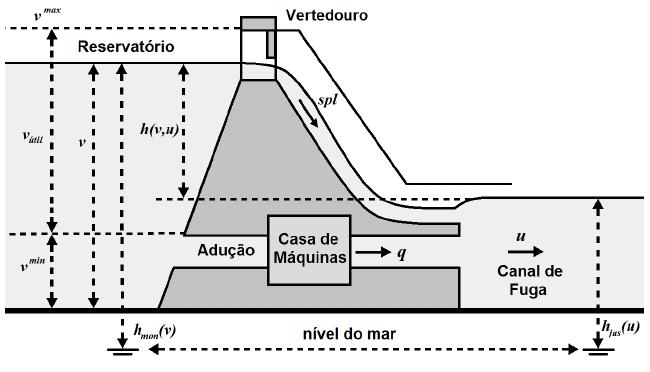
\includegraphics[width=2.5in]{./fig/Componentes-usinas-hidreletricas.jpg}
  \label{fig:componentesUsinasHidreletricas}
\end{figure}

\begin{description}[\IEEEsetlabelwidth{$h_{jus}(u)$}]
 \item[$v$] volume do reservat�rio [$hm^{3}$]
 \item[$v^{max}$] volume m�ximo operativo do reservat�rio [$hm^{3}$]
 \item[$v^{min}$] volume m�nimo operativo do reservat�rio [$hm^{3}$]
 \item[$v_{util}$] volume �til do reservat�rio ($v^{max} - v^{min}$) [$hm^{3}$]
 \item[$q$] vaz�o turbinada pela casa de m�quinas (engolimento) [$m^{3}/s$]
 \item[$spl$] vaz�o descarregada pelo vertedouro (vertimento) [$m^{3}/s$]
 \item[$u$] vaz�o descarregada pela usina (deflu�ncia) ($q + spl$) [$m^{3}/s$]
 \item[$h_{mon}(v)$] cota de montante do reservat�rio (fun��o do volume) [$m$]
 \item[$h_{jus}(u)$] cota de jusante do reservat�rio (fun��o da deflu�ncia) [$m$]
 \item[$h(v, u)$] altura de queda l�quida ($h_{mon}(v) - h_{jus}(u)$) [$m$]
\end{description}

Vale notar que a vari�vel $q$, a qual representa a vaz�o turbinada, � limitada pelo engolimento m�ximo da usina $q^{max}$, que � a vaz�o turbinada capaz de produzir a pot�ncia m�xima da usina para uma data altura de queda.

Em um mesmo rio, � comum a constru��o de uma cascata de usinas hidrel�tricas. Dessa forma, a vaz�o descarregada da usina anterior, conhecida como montante, ir� para o reservat�rio da usinas posterior, conhecida como jusante. Essa vaz�o poder� passar novamente por regulariza��o no reservat�rio da usina em jusante.

\subsection{Formula��o do Problema de Planejamento da Opera��o Energ�tica}

O planejamento da opera��o energ�tica tem como objetivo minimizar o custo de gera��o de um sistema termel�trico, ao mesmo tempo que mant�m os reservat�rios das usinas hidrel�tricas em alta. Ou seja, temos aqui dois objetivos distintos: minimizar o custo, o qual tem sua por��o vari�vel na gera��o t�rmica complementar, e maximizar o volume final dos reservat�rios. Para resolver esse problema, consideram-se conhecidas as vaz�es afluentes e a demanda e leva-se em conta as caracter�sticas individuais de cada usina hidrel�trica. As fun��es objetivos a serem otimizadas s�o descritas pelo vetor objetivo $\vec{F}$ mostrado na Equa��o \ref{eq:funcoesObjetivo}, onde $CT$ representa a soma dos custos de gera��o de energia por usinas t�rmicas durante todo o per�odo de planejamento (Equa��o \ref{eq:funcaoObjetivoCustoTermico}) e $VF$ � associada ao n�vel dos reservat�rios das hidrel�tricas no �ltimo per�odo de planejamento.

\begin{equation}\label{eq:funcoesObjetivo}
 \vec{F} = \{CT, VF\}
\end{equation}

O parque termel�trico � considerado como se toda a gera��o el�trica se concentrasse em uma �nica usina, isso se d� pela impossibilidade de se poder atribuir um custo preciso � opera��o da gera��o t�rmica sem considerar diversos outros fatores. Portanto, utiliza-se uma fun��o polinomial para representar o custo da gera��o da energia el�trica, como exibido na Equa��o \ref{eq:custoTermico}.

\begin{equation}\label{eq:funcaoObjetivoCustoTermico}
 CT = min \sum_{t=1}^{T} f(gt_{t})
\end{equation}

\begin{equation}\label{eq:custoTermico}
 f(gt_{t}) = \alpha + \beta.gt_{t} + \gamma.gt_{t}^{2} 
\end{equation}

As fun��es objetivos est�o sujeitas �s seguintes restri��es:

\begin{equation}\label{eq:balanceamentoDeCarga}
 gt_{t} + \sum_{i=1}^{N} gh_{it} - D_{t} - L_{t} = 0
\end{equation}

\begin{equation}\label{eq:limitesGeracaoTermica}
 gt^{min} \leq gt_{t} \leq gt^{max}
\end{equation}

\begin{equation}\label{eq:limitesGeracaoHidreletrica}
 gh_{i}^{min} \leq gh_{it} \leq gh_{i}^{max}
\end{equation}

\begin{equation}\label{eq:geracaoHidraulica}
 gh_{it} = k_{i}.[h_{mon}(v_{it}) - h_{jus}(q_{it} + spl_{i}) - pc].q_{it}
\end{equation}

\begin{equation}\label{eq:balanceamentoDinamicoDaAgua}
 v_{it} = v_{i,t-1} + y_{it} - q_{it} - spl_{it} + \sum_{m=1}^{\Phi_{i}} (q_{m,t} + spl_{m,t}), m \in \Phi_{i}
\end{equation}

\begin{equation}\label{eq:limitesArmazenamento}
 v_{i}^{min} \leq v_{it} \leq v_{i}^{max}
\end{equation}

\begin{equation}\label{eq:volumeInicial}
 v_{i0} = v_{i}^{ini}
\end{equation}

\begin{equation}\label{eq:volumeFinal}
 v_{iT} = v_{i}^{final}
\end{equation}

\begin{equation}\label{eq:limitesTurbinagem}
 q_{i}^{min} \leq q_{it} \leq q_{i}^{max}(h_{i}(t))
\end{equation}

onde: 

\begin{description}[\IEEEsetlabelwidth{$h_{jus}(q_{it} + spl_{it})$}]
 \item[$F$] custo t�rmico total durante o horizonte [\$]
 \item[$T$] n�mero de est�gios do horizonte de planejamento (intervalo de tempo) [meses]
 \item[$t$] �ndice do intervalo de tempo [m�s]
 \item[$N$] n�mero de usinas do sistema
 \item[$i$] �ndice da usina do sistema
 \item[$gt_{t}$] gera��o termel�trica durante o intervalo $t$ [$\overline{\rm MW}$\footnote{Um $\overline{\rm MW}$ � a energia correspondente a uma fonte de um $MW$ de pot�ncia em dado per�odo. Neste caso, o per�odo considerado � de um m�s.}]
 \item[$f(gt_{t})$] fun��o de custo de gera��o t�rmica no instante $t$ [\$]
 \item[$gh_{it}$] gera��o da usina $i$ durante o per�odo $t$ [$\overline{\rm MW}$]
 \item[$v_{it}$] volume do reservat�rio da usina $i$ no final do intervalo $t$ [$hm^{3}$]
 \item[$q_{it}$] vaz�o turbinada pela usina $i$ durante o intervalo $t$ [$m^{3}$]
 \item[$spl_{it}$] vaz�o vertida pela usina $i$ durante o intervalo $t$ [$m^{3}$]
 \item[$k_{it}$] produtibilidade da usina $i$
 \item[$h_{mon}(v_{it})$] fun��o da cota do montante do reservat�rio da usina $i$ no instante $t$ [$m$]
 \item[$h_{jus}(q_{it} + spl_{it})$] fun��o da cota do jusante do reservat�rio da usina $i$ no instante $t$ [$m$]
 \item[$pc$] perdas hidr�ulicas
 \item[$y_{it}$] vaz�o incremental afluente � usina $i$ durante o intervalo $t$ [$m^{3}/s$]
 \item[$\Phi_{i}$] conjunto de usinas imediatamente a montante da usina $i$
 \item[$D_{t}$] mercado (demanda) a ser atendido durante o per�odo $t$ [$\overline{\rm MW}$]
 \item[$L_{t}$] perdas na transmiss�o de energia no instante $t$ [$\overline{\rm MW}$]
 \item[$\alpha, \beta, \gamma$] coeficientes da fun��o custo de gera��o t�rmica
 \item[$v_{i}^{min},v_{i}^{max}$] volume m�nimo e m�ximo do reservat�rio da usina $i$ [$hm^{3}$]
 \item[$v_{i}^{ini},v_{i}^{final}$] volume inicial e final do reservat�rio da usina $i$ [$hm^{3}$]
 \item[$q_{i}^{min},q_{i}^{max}$] turbinagem m�nima e m�xima da usina $i$ [$m^{3}$]
 \item[$gh_{i}^{min},gh_{i}^{max}$] capacidade m�nima e m�xima de gera��o hidr�ulica da usina $i$ [$\overline{\rm MW}$]
 \item[$gt_{i}^{min},gt_{i}^{max}$] capacidade m�nima e m�xima de gera��o t�rmica [$\overline{\rm MW}$]
 \item[$h_{i}(t)$] altura de queda da usina $i$ no instante $t$ [$m$]
\end{description}

\section{Sistemas Hidrot�rmicos de Gera��o}
\label{cap:sistemasHidrotermicos}

Em um sistema hidrot�rmico de gera��o, como o encontrado no cen�rio Brasileiro, existem dois meios majorit�rios de gera��o de energia el�trica: atrav�s de usinas hidrel�tricas, as quais utilizam a energia de quedas hidr�ulicas, e usinas termel�tricas, as quais fazem queima de combust�veis f�sseis ou fiss�o nuclear. A energia el�trica gerada atrav�s desses meios � transmitida para os mercados consumidores atrav�s de linhas de transmiss�o e distribui��o.

Os custos envolvidos nessa gera��o de energia dependem da fonte utilizada. No caso da energia gerada atrav�s de usinas hidrel�tricas, existe apenas o custo de manuten��o e opera��o das m�quinas, o qual n�o depende da quantidade de energia gerada. Portanto, essas apresentam custo fixo. Enquanti isso, ao produzir energia atrav�s de usinas termel�tricas, o custo de gera��o depende do pre�o e quantidade dos combust�veis utilizados. Essa quantidade varia de acordo com a quantidade de energia gerada, caracterizando um custo vari�vel.

Devido ao alto custo de combust�veis utilizados na gera��o el�trica, d�-se prefer�ncia � gera��o atrav�s de usinas hidrel�tricas, que apresentam custos fixos e inferiores. Entretanto, essas n�o s�o capazes de gerar 100\% da energia necess�ria o tempo todo, visto que t�m produtividade que varia de acordo com fen�menos naturais. Ent�o, a estrat�gia utilizada � de se gerar energia primariamente atrav�s das usinas hidrel�tricas e se complementar com as usinas termel�tricas. A seguir, detalhamos o funcionamento de ambos tipos de usinas.

\subsection{Usinas Hidrel�tricas}

O processo de gera��o de energia hidrel�trica baseia-se na transforma��o de energia potencial hidr�ulica, gerada pela diferen�a de altura, em energia el�trica. O processo se inicia com o armazenamento de �gua dos rios em reservat�rios ou lagos, atrav�s da constru��o de obras de represamento. A principal fun��o da represa � criar a diferen�a de altura, provocando o ac�mulo de energia hidr�ulica. A �gua do reservat�rio � conduzida
sob press�o atrav�s de condutos for�ados at� o conjunto de turbinas da usina, denominado casa de m�quinas. Na casa de m�quinas, a �gua � utilizada para impulsionar as p�s (ou l�minas) das turbinas. A energia cin�tica e a energia de press�o din�mica desenvolvida no percurso da �gua, atrav�s das tubula��es, s�o convertidas em energia cin�tica de rota��o. As turbinas est�o ligadas a geradores que, postos em movimento cont�nuo, convertem a energia cin�tica em energia el�trica. Depois de passar pelas turbinas, a �gua retorna ao rio atrav�s de canais ou condutos, pelo chamado canal de fuga da usina. \cite{silva2014}

Al�m disso, � poss�vel a libera��o da �gua sem que essa passe pelas turbinas. Isso se d� atrav�s do vertedouro. O objetivo � controlar o n�vel do reservat�rio quando h� mais �gua do que a usina consegue utilizar na gera��o de energia. O problema disso � que a �gua que passa pelo vertedouro pode ser considerada energia desperdi�ada, j� que a fonte de energia da usina � a �gua existente em seu reservat�rio.

Para que a energia gerada possa ser calculada, utiliza-se de um modelo matem�tica da usina. Esse modelo � uma fun��o de gera��o que relaciona vari�veis mensur�veis � energia gerada. Como entrada, esse modelo requer as seguintes vari�veis: volume de �gua armazenado no reservat�rio, vaz�o turbinada e vaz�o vertida. Atrav�s delas,  � poss�vel calcular a quantidade de energia gerada, como sugere a Figura \ref{fig:modeloHidreletrica}.

\begin{figure}[!t]
  \centering
  \caption{Vari�veis de entrada e sa�da utilizadas no Modelo geral de uma Usina Hidroel�trica}
  \includegraphics[width=2.5in]{./fig/Modelo-Hidreletrica.pdf}
  \label{fig:modeloHidreletrica}
\end{figure}

Naturalmente, esse modelo matem�tico depende de outras vari�veis al�m das vari�veis de entrada. Portanto, estudaremos a seguir os principais componentes de uma usina hidrel�trica, como mostrado na Figura \ref{fig:componentesUsinasHidreletricas}.

\begin{figure}[!t]
  \centering
  \caption{Principais componentes de uma Usina Hidrel�trica \cite{silva2014}}
  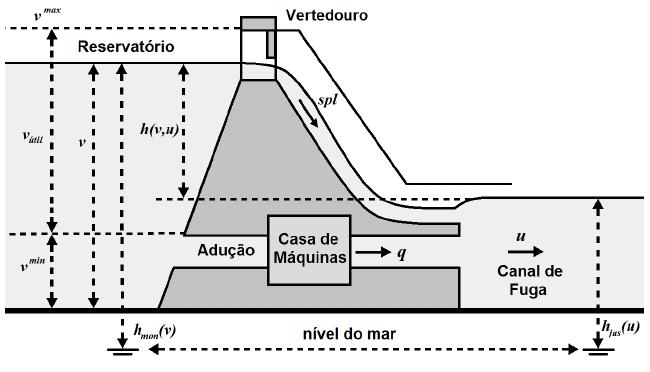
\includegraphics[width=2.5in]{./fig/Componentes-usinas-hidreletricas.jpg}
  \label{fig:componentesUsinasHidreletricas}
\end{figure}

\begin{description}
 \item[$v$] volume do reservat�rio [$hm^{3}$]
 \item[$v^{max}$] volume m�ximo operativo do reservat�rio [$hm^{3}$]
 \item[$v^{min}$] volume m�nimo operativo do reservat�rio [$hm^{3}$]
 \item[$v_{�til}$] volume �til do reservat�rio ($v^{max} - v^{min}$) [$hm^{3}$]
 \item[$q$] vaz�o turbinada pela casa de m�quinas (engolimento) [$m^{3}/s$]
 \item[$spl$] vaz�o descarregada pelo vertedouro (vertimento) [$m^{3}/s$]
 \item[$u$] vaz�o descarregada pela usina (deflu�ncia) ($q + spl$) [$m^{3}/s$]
 \item[$h_{mon}(v)$] cota de montante do reservat�rio (fun��o do volume) [$m$]
 \item[$h_{jus}(u)$] cota de jusante do reservat�rio (fun��o da deflu�ncia) [$m$]
 \item[$h(v, u)$] altura de queda l�quida ($h_{mon}(v) - h_{jus}(u)$) [$m$]
\end{description}

Vale notar que a vari�vel $q$, a qual representa a vaz�o turbinada, � limitada pelo engolimento m�ximo da usina $q^{max}$, que � a vaz�o turbinada que produzir a pot�ncia m�xima da usina para uma data altura de queda.

\subsubsection{Reservat�rios}

O reservat�rio de uma usina hidrel�trica � respons�vel por armazenar a �gua que ser� utilizada na gera��o el�trica. Eles s�o classificados em duas categorias: de compensa��o e de acumula��o. Enquanto os reservat�rios de compensa��o t�m volume o suficiente apenas para regulariza��o de cargas semanais ou mensais, os de acumula��o s�o capazes de regularizar vaz�es de alguns meses a alguns anos, tudo isso dependendo de seu volume. Por regularizar, entende-se a capacidade de atenuar a varia��o da disponibilidade de �gua, tornando poss�vel a utilizando de �gua proveniente de um per�odo de chuvas em um per�odo de estiagem. Vale notar que em horizontes de planejamento de m�dio e longo prazo, a capacidade de regulariza��o de usinas fio d'�gua, aquelas com reservat�rio de compensa��o, s�o desprezadas.

Em um mesmo rio, � comum a constru��o de uma cascata de usinas hidrel�tricas. Dessa forma, a vaz�o descarregada da usina anterior, conhecida como montante, ir� para o reservat�rio da usinas posterior, conhecida como jusante. Essa vaz�o poder� passar novamente por regulariza��o no reservat�rio da usina em jusante. A Figura \ref{fig:cascataUsinas} ilusta uma cascata de usinas localizadas no sistema sudeste. As usinas com reservat�rio de acumula��o s�o representadas pelo s�mbolo triangular, enquanto as usinas com reservat�rio de compensa��o s�o representadas pelo s�mbolo circular.

\begin{figure}[!t]
  \centering
  \caption{Cascata de usinas localizadas no sistema sudeste}
  \includegraphics[width=2.5in]{./fig/Cascata-Usinas.pdf}
  \label{fig:cascataUsinas}
\end{figure}

\subsubsection{Conjuntos Turbina/Gerador}

\subsection{Usinas Termel�tricas}

\subsection{Formula��o do Problema de Planejamento da Opera��o Energ�tica}

O planejamento da opera��o energ�tica tem como objetivo minimizar o custo de gera��o de um sistema termel�trico, ao mesmo tempo que mant�m os reservat�rios das usinas hidrel�tricas em alta. Ou seja, temos aqui dois objetivos distintos: minimizar o custo, o qual tem sua por��o vari�vel na gera��o t�rmica complementar, e maximizar o volume final dos reservat�rios. Para resolver esse problema, consideram-se conhecidas as vaz�es afluentes e a demanda e leva-se em conta as caracter�sticas individuais de cada usina hidrel�trica. As fun��es objetivos a serem otimizadas s�o descritas pelo vetor objetivo $\vec{F}$ mostrado na Equa��o \ref{eq:funcoesObjetivo}, onde $CT$ representa a soma dos custos de gera��o de energia por usinas t�rmicas durante todo o per�odo de planejamento (Equa��o \ref{eq:funcaoObjetivoCustoTermico}) e $VF$ � associada ao n�vel dos reservat�rios das hidrel�tricas no �ltimo per�odo de planejamento.

\begin{equation}\label{eq:funcoesObjetivo}
 \vec{F} = \{CT, VF\}
\end{equation}

O parque termel�trico � considerado como se toda a gera��o el�trica se concentrasse em uma �nica usina, isso se d� pela impossibilidade de se poder atribuir um custo preciso � opera��o da gera��o t�rmica sem considerar diversos outros fatores, como por exemplo, o pre�o atual dos combust�veis utilizados e o tipo de usina. Portanto, utiliza-se uma fun��o polinomial para representar o custo da gera��o da energia el�trica, como exibido na Equa��o \ref{eq:custoTermico}.

\begin{equation}\label{eq:funcaoObjetivoCustoTermico}
 CT = min \sum_{t=1}^{T} f(gt_{t})
\end{equation}

\begin{equation}\label{eq:custoTermico}
 f(gt_{t}) = \alpha + \beta.gt_{t} + \gamma.gt_{t}^{2} 
\end{equation}

As fun��es objetivos est�o sujeitas �s seguintes restri��es:

\begin{equation}\label{eq:balanceamentoDeCarga}
 gt_{t} + \sum_{i=1}^{N} gh_{it} - D_{t} - L_{t} = 0
\end{equation}

\begin{equation}\label{eq:limitesGeracaoTermica}
 gt^{min} \leq gt_{t} \leq gt^{max}
\end{equation}

\begin{equation}\label{eq:limitesGeracaoHidreletrica}
 gh_{i}^{min} \leq gh_{it} \leq gh_{i}^{max}
\end{equation}

\begin{equation}\label{eq:geracaoHidraulica}
 gh_{it} = k_{i}.[h_{mon}(v_{it}) - h_{jus}(q_{it} + spl_{i}) - pc].q_{it}
\end{equation}

\begin{equation}\label{eq:balanceamentoDinamicoDaAgua}
 v_{it} = v_{i,t-1} + y_{it} - q_{it} - spl_{it} + \sum_{m=1}^{\Phi_{i}} (q_{m,t} + spl_{m,t}), m \in \Phi_{i}
\end{equation}

\begin{equation}\label{eq:limitesArmazenamento}
 v_{i}^{min} \leq v_{it} \leq v_{i}^{max}
\end{equation}

\begin{equation}\label{eq:volumeInicial}
 v_{i0} = v_{i}^{ini}
\end{equation}

\begin{equation}\label{eq:volumeFinal}
 v_{iT} = v_{i}^{final}
\end{equation}

\begin{equation}\label{eq:limitesTurbinagem}
 q_{i}^{min} \leq q_{it} \leq q_{i}^{max}(h_{i}(t))
\end{equation}

onde: 

\begin{description}
 \item[$F$] custo t�rmico total durante o horizonte [\$]
 \item[$T$] n�mero de est�gios do horizonte de planejamento (intervalo de tempo) [meses]
 \item[$t$] �ndice do intervalo de tempo [m�s]
 \item[$N$] n�mero de usinas hidrel�tricas do sistema
 \item[$i$] �ndice da usina hidrel�trica do sistema
 \item[$gt_{t}$] gera��o termel�trica durante o intervalo $t$ [$\overline{\rm MW}$\footnote{Um $\overline{\rm MW}$ � a energia correspondente a uma fonte de um $MW$ de pot�ncia em dado per�odo. Neste caso, o per�odo considerado � de um m�s.}]
 \item[$f(gt_{t})$] fun��o de custo de gera��o t�rmica no instante $t$ [\$]
 \item[$gh_{it}$] gera��o da usina hidrel�trica $i$ durante o per�odo $t$ [$\overline{\rm MW}$]
 \item[$v_{it}$] volume do reservat�rio da usina hidrel�trica $i$ no final do intervalo $t$ [$hm^{3}$]
 \item[$q_{it}$] vaz�o turbinada pela usina hidrel�trica $i$ durante o intervalo $t$ [$m^{3}$]
 \item[$spl_{it}$] vaz�o vertida pela usina hidrel�trica $i$ durante o intervalo $t$ [$m^{3}$]
 \item[$k_{it}$] produtibilidade da usina hidrel�trica $i$
 \item[$h_{mon}(v_{it})$] fun��o da cota do montante do reservat�rio da usina hidrel�trica $i$ no instante $t$ [$m$]
 \item[$h_{jus}(q_{it} + spl_{it})$] fun��o da cota do jusante do reservat�rio da usina hidrel�trica $i$ no instante $t$ [$m$]
 \item[$pc$] perdas hidr�ulicas
 \item[$y_{it}$] vaz�o incremental afluente � usina hidrel�trica $i$ durante o intervalo $t$ [$m^{3}/s$]
 \item[$\Phi_{i}$] conjunto de usinas imediatamente a montante da usina $i$
 \item[$D_{t}$] mercado (demanda) a ser atendido durante o per�odo $t$ [$\overline{\rm MW}$]
 \item[$L_{t}$] perdas na transmiss�o de energia no instante $t$ [$\overline{\rm MW}$]
 \item[$\alpha, \beta, \gamma$] coeficientes da fun��o custo de gera��o t�rmica
 \item[$v_{i}^{min},v_{i}^{max}$] volume m�nimo e m�ximo do reservat�rio da usina hidrel�trica $i$ [$hm^{3}$]
 \item[$v_{i}^{ini},v_{i}^{final}$] volume inicial e final do reservat�rio da usina hidrel�trica $i$ [$hm^{3}$]
 \item[$q_{i}^{min},q_{i}^{max}$] turbinagem m�nima e m�xima da usina hidrel�trica $i$ [$m^{3}$]
 \item[$gh_{i}^{min},gh_{i}^{max}$] capacidade m�nima e m�xima de gera��o hidr�ulica da usina hidrel�trica $i$ [$\overline{\rm MW}$]
 \item[$gt_{i}^{min},gt_{i}^{max}$] capacidade m�nima e m�xima de gera��o t�rmica [$\overline{\rm MW}$]
 \item[$h_{i}(t)$] altura de queda da usina hidrel�trica $i$ no instante $t$ [$m$]
\end{description}

Essas f�rmulas matem�ticas descrevem o comportamento do conjunto de usinas em um planejamento de m�dio prazo e s�o auto explicativas. Vale observar que algumas caracter�sticas, que seriam importantes em um planejamento de curto prazo, puderam ser ignoradas aqui. Por exemplo, em uma discretiza��es hor�rias, deve-se levar em conta a diferen�a de tempo que a vaz�o de uma usina a montante leva para chegar ao reservat�rio da usina � jusante. Entretanto, com uma discretiza��o mensal, isso pode ser ignorado.

Dentre as equa��es apresentadas, vale a pena destacar algumas equa��es para tornar a formula��o mais clara. A equa��o \ref{eq:balanceamentoDeCarga}, que � conhecida como equa��o de balanceamento de carga e representa o balan�o entre produ��o t�rmica ($gt$) e hidr�ulica ($gh$) para atender � demanda $D$, considerando as perdas de carga $L$ na transmiss�o. J� o balanceamento din�mico de �gua, apresentado pela equa��o \ref{eq:balanceamentoDinamicoDaAgua}, garante o correto equil�brio entre a �gua que entra e sai da usina. Ela indica que o volume do reservat�rio de uma usina num determinado instante $t$ � o volume que ela possu�a no instante anterior, somado ao que recebeu de �gua (seja vaz�o incremental ou oriunda das usinas � montante), subtra�do o que ela devolveu de �gua ao sistema (seja turbinada ou vertida). As demais equa��es descrevem os c�lculos de gera��o t�rmica e hidrel�trica, al�m de especificar as restri��es do sistema.
\section{Descrição dos Algoritmos Avaliados}
\label{cap:sistemasHidrotermicos} 

\section{Estudos de Caso}
\label{cap:estudosDeCaso}

Foram implementados alguns dos mais eficientes algoritmos de otimiza��o multiobjetivo encontrados na literatura atual na solu��o do Problema do Planejamento Energ�tico de Sistemas Hidrot�rmicos. Tr�s deles s�o baseados em algoritmos evolucion�rios: NSGA-II \cite{deb2002}, SPEA2 \cite{zitzler2001} e MOCell \cite{nebro2006} \cite{nebro2007}; e dois s�o baseados em enxame de part�culas: OMOPSO \cite{reyes2005} e SMPSO \cite{nebro2009}. Ap�s m�ltiplas execu��es desses algoritmos, seus resultados foram comparados a fim de se encontrar a melhor t�cnica para a solu��o do problema.

\subsection{Cen�rio de Teste}

O problema do planejamento energ�tico foi simulado para um conjunto de 8 usinas hidrel�tricas reais do sistema brasileiro, utilizando dados reais de tr�s per�odos de 60 meses: maio/1951 a abril/1956, maio/1961 a abril/1966 e maio/1980 a abril/1985. As usinas est�o localizadas na Bacia do Rio Grande e Parana�ba. Elas est�o esquematizadas na Figura \ref{fig:conjuntoUsinas} e suas caracter�sticas s�o apresentadas na Tabela \ref{table:conjuntoUsinas}. Os tr�s per�odos utilizadados aqui, tamb�m foram utilizados em \cite{gomides2012} e \cite{silva2014} devido �s suas caracter�sticas �nicas e relevantes para a otimiza��o. O primeiro per�odo � determinado por meses de seca, a vaz�o dos rios estava baixa e o custo de gera��o el�trica consequentemente se tornou maior, esse � o per�odo mais importante utilizado neste estudo de caso, uma vez que � o que mais apresenta restri��es � otimiza��o do problema. O segundo e o terceiro per�odo s�o caracterizados por vaz�es m�dias e altas dos rios, respectivamente.

\begin{figure}[!t]
  \centering
  \caption{Topologia usada no Estudo de Caso}
  \includegraphics[width=2.5in]{./fig/Conjunto-Usinas.pdf}
  \label{fig:conjuntoUsinas}
\end{figure}

\begin{table}[!t]
\caption{Conjunto de Usinas Hidrel�tricas estudadas}
\label{table:conjuntoUsinas}
\centering
\begin{tabular}{lcc}
    \hline
    Usina                 & Pot�ncia (MW)  & Reservat�rio (hm$^{3}$)  \\ \hline
    Furnas                & $1,312$        & $22,950$                 \\
    Mascarenhas de Moraes & $478$          & $4,040$                  \\
    Marimbondo            & $1,488$        & $6,150$                  \\
    �gua Vermelha         & $1,396.2$      & $11,025$                 \\
    Emborca��o            & $1,192$        & $17,725$                 \\
    Itumbiara             & $2,280$        & $17,027$                 \\
    S�o Sim�o             & $1,710$        & $12,540$                 \\
    Ilha Solteira         & $3,444$        & $21,046.359375$          \\ \hline
    Total                 & $13,300.2$     & $112,503.359375$         \\ \hline
\end{tabular}
\end{table}

Os estudos de casos precisam simular o atendimento da demanda por energia el�trica mensal, essa demanda de mercado ($D_{t}$) deve ser atendida pela combina��o das gera��es hidr�ulicas e t�rmicas. No Brasil, a EPE realiza estudos e determina, anualmente, a previs�o de demanda para todo o Sistema Interligado Nacional para os pr�ximos 10 anos. Entretanto, para simplificar o processo de simula��o, a demanda foi considerada constante e com valor igual ao arredondado para cima da pot�ncia total das 8 usinas: $D_{t} = 14,000$. O mesmo valor foi utilizado nos estudos de \cite{gomides2012} e \ref{silva2014}. Em rela��o �s chuvas e vaz�es, optou-se pela utiliza��o de dados reais dos per�odos citados. Assim, � poss�vel calcular a gera��o hidrel�trica, obter a gera��o t�rmica necess�ria para se complementar a demanda e por fim calcular o custo t�rmico.

Para o c�lculo do custo t�rmico ($CT$), utilizou-se a Equa��o \ref{eq:calculoCustoTermico}, onde $gt_{t}$ representa a gera��o t�rmica total. Essa equa��o � uma adapta��o da Equa��o \ref{}, onde $\alpha = \beta = 0$ e $\gamma = \frac{1}{2}$.

\begin{equation}\label{eq:calculoCustoTermico}
 CT = f(gt_{t}) = \frac{1}{2}(gt_{t})^{2}
\end{equation} 

\subsection{Arquitetura do Sistema}

Para implementa��o dos algoritmos, foi utilizada a linguagem Java em conjunto com o framework JMetal \cite{durillo2011}, o qual disponibiliza diversos algoritmos de otimiza��o orientados a objetos e toda um l�gica de execu��o dos estudos com a cria��o de um relat�rio dos resultados ao fim. Seguindo a API desse framework, cada part�cula do enxame/elemento da popula��o foi implementada como um $DoubleSolution$, o qual � um objeto contendo um vetor de n�meros reais. Para o problema apresentado, cada poss�vel solu��o foi composta por um vetor de 480 n�meros reais, os quais possuiam valores entre 0 e 1. Esses valores representam a turbinagem normalizada de determinada usina do conjunto em determinado m�s dentro do per�odo. Como cada per�odo possui 60 meses e existem 8 usinas nesse estudo de caso, o vetor foi organizado em grupos de 60 n�mero reais representando a turbinagem normalizada, totalizando os 480 n�meros reais. Vale notar que a normaliza��o dessa turbinagem ocorre atrav�s da divis�o da quantidade turbinada pelo engolimento m�ximo da usina correspondente.

Com essa composi��o das poss�veis solu��es, torna-se poss�vel os c�lculos que levam �s duas vari�veis a serem otimizadas: custo de opera��o e armazenamento final dos reservat�rios. Esses c�lculos foram executados para cada part�cula do enxame/elemento da popula��o pelo simulador de opera��o de usinas hidrel�tricas disponibilizado por \cite{ramos2017}. Esse simulador possui um banco de dados com os dados das usinas hidrel�tricas estudadas, bem como os dados de aflu�ncias ocorridas nos per�odos do estudo. Assim, atrav�s da turbinagem de cada usina em cada m�s em conjunto com os dados de aflu�ncias, ele � capaz de calcular diversos resultados para aquele m�s, como a pot�ncia gerada, vertimento, armazenamento ao fim do m�s, entre outros. O simulador automaticamente reutiliza esses resultados para o c�lculo dos meses seguintes e tamb�m das usinas a jusante. Assim, ele retorna os resultados de todos os meses de todas as usinas para dada simula��o. Por fim, utiliza-se a pot�ncia total gerada e a demanda para o c�lculo do custo de gera��o t�rmica (a ser minimizada) e soma-se o armazenamento final de todas as usinas (a ser maximizado).

Para a execu��o dos algoritmos, foi utilizada uma m�quina virtual da Linode com seis n�cleos do processador Intel E5-2680v3 de 2.5GHz, 12GB de mem�ria RAM e sistema operacional Ubuntu 16 de 64bit. O execut�vel do c�digo fonte era gerado pelo Maven e esse c�digo teve versionamento atrav�s do Git. Assim, o execut�vel era enviado para a m�quina virtual, onde poderia rodar 24h por dia at� sua conclus�o. Por seguran�a, foi criado um esquema que permitia que a execu��o pudesse continuar de onde parou, caso acontecesse alguma interrup��o.

\subsection{Par�metros Utilizados nos Algoritmos}
\label{sec:parametrosUtilizados}

Com o fim de tornar a compara��o entre esses algoritmos mais justa, foram utilizados os par�metros exibidos na Tabela \ref{table:parametrosUtilizados}. Esses foram os mesmos utilizados na avalia��o desses mesmos algoritmos (com a adi��o do AbYSS) feita por \cite{nebro2009} atrav�s de conhecidos benchmarks. Vale notar que o fato de determinado algoritmo ter melhores resultados em certo benchmark n�o indica que ele ser� melhor em todos problemas reais. Portanto, espera-se obter diferentes resultados na solu��o do Problema do Planejamento Energ�tico de Sistemas Hidrot�rmicos.

\begin{table}[!t]
\caption{Par�metros utilizados nos Algoritmos ($L$ = tamanho do indiv�duo)}
\label{table:parametrosUtilizados}
\centering
\begin{tabular}{ll}
    \hline
    \multicolumn{2}{l}{Par�metros utilizados no NSGA-II}                     \\ \hline
    Tamanho da Popula��o           & 100 indiv�duos                          \\
    Sele��o de Pais                & torneio bin�rio + torneio bin�rio       \\
    Recombina��o                   & bin�ria simulada (SBX), $p_{c} = 0.9$   \\
    Muta��o                        & polinomial, $p_{m} = 1.0/L$             \\
    \hline
    \multicolumn{2}{l}{Par�metros utilizados no SPEA2}                       \\ \hline
    Tamanho da Popula��o           & 100 indiv�duos                          \\
    Sele��o de Pais                & torneio bin�rio + torneio bin�rio       \\
    Recombina��o                   & bin�ria simulada (SBX), $p_{c} = 0.9$   \\
    Muta��o                        & polinomial, $p_{m} = 1.0/L$             \\
    \hline
    \multicolumn{2}{l}{Par�metros utilizados no MOCell}                      \\ \hline
    Tamanho da Popula��o           & 100 indiv�duos (10 x 10)                \\
    Vizinhan�a                     & 1 salto (8 solu��es em torno)           \\
    Sele��o de Pais                & torneio bin�rio + torneio bin�rio       \\
    Recombina��o                   & bin�ria simulada (SBX), $p_{c} = 0.9$   \\
    Muta��o                        & polinomial, $p_{m} = 1.0/L$             \\
    Tamanho do Arquivo             & 100 indiv�duos                          \\
    \hline
    \multicolumn{2}{l}{Par�metros utilizados no OMOPSO}                      \\ \hline
    Tamanho do Enxame              & 100 part�culas                          \\
    Muta��o                        & uniforme + n�o uniforme                 \\
    Tamanho dos L�deres            & 100                                     \\
    \hline
    \multicolumn{2}{l}{Par�metros utilizados no SMPSO}                       \\ \hline
    Tamanho do Enxame              & 100 part�culas                          \\
    Muta��o                        & polinomial, $p_{m} = 1.0/L$             \\
    Tamanho do Arquivo             & 100 indiv�duos                          \\
    \hline
\end{tabular}
\end{table}

Al�m desses par�metros, existe um par�metro impl�cito utilizado na muta��o polinomial e na recombina��o bin�ria simulada (SBX), operadores presentes em todos os algoritmos, com exce��o do OMOPSO que n�o possui esses operadores e o SMPSO que possui apenas a muta��o polinomial. Esse par�metro � chamado de �ndice de distribui��o, possui valor real acima de $0$ e geralmente assume o valor padr�o de $20.0$. Esse �ndice trabalha nesses operadores de muta��o e recombina��o de tal forma que, quanto menor seu valor, maior ser� a diversidade dos novos indiv�duos criados, aumentando a explora��o do ambiente por parte dos algoritmos de busca. Para este trabalho, tr�s valores diferentes foram adotados na avalia��o dos algoritmos: $1.0$, $10.0$ e $20.0$. Dessa forma, cada algoritmo (que possua esse par�metro) foi avaliado tr�s vezes distintas, cada uma com um desses valores de �ndice de distribui��o.

Por fim, os algoritmos testados continham uma popula��o de 100 part�culas/indiv�duos, como mostrado na Tabela \ref{table:parametrosUtilizados}, e cada execu��o continha 500 itera��es. Foram realizadas 25 execu��es de cada par de algoritmo e �ndice de distribui��o para cada periodo considerado neste trabalho.

\section{Resultados e Discuss�es}
\label{cap:resultadosDiscussoes}

Deseja-se avaliar os resultados obtidos por esses algoritmos de acordo com os dois objetivos utilizados: diminuir os custos de gera��o t�rmica e aumentar o armazenamento final dos reservat�rios das usinas. Para facilitar a visualiza��o das frentes de pareto, o armazenamento final foi convertido em porcentagem, indo de 0 a 100\%. Al�m disso, os valores do armazenamento final receberam valores negativos, sendo apresentados de -100 at� 0\%.

Os valores obtidos pelos algoritmos utilizados ser�o comparados entre si atrav�s de conhecidas m�tricas de qualidade, al�m da apresenta��o dos gr�ficos de suas frentes de pareto junto � frente de refer�ncia. Deve-se notar que, por n�o possuirmos uma frente de pareto de refer�ncia ideal com o melhor resultado poss�vel, foi criada uma a partir dos melhores resultados de todas execu��es de todos os algoritmos.

Tamb�m � importante notar que devido �s diferen�as de configura��o das oito usinas adotadas devido ao uso de um simulador de terceiro que n�o permitia altera��o dessas configura��es, os n�meros obtidos aqui n�o s�o compar�veis com os dois estudos realizados em \cite{gomides2012} e \cite{silva2014}.

\subsection{Per��odo 1951-1956}

Tratando-se de um per�odo de seca, espera-se maior dificuldade na otimiza��o da opera��o das usinas nesse per�odo. Portanto, � um per�odo chave na compara��o entre os algoritmos.

A Tabela \ref{table:epPeriodo1} apresenta a mediana e o desvio do valor do Indicador Epsilon Aditivo (\textit{I}$^{1}_{\epsilon+}$) obtido em todas execu��es de cada algoritmo para esse per�odo. Esse indicador mostra o qu�o pr�xima a frente de pareto obtida est� da verdadeira frente de pareto (nesse caso, como j� citado, obtida com os melhores resultados de todos algoritmos), sendo melhor o resultado quanto menor o valor. Nessa tabela tamb�m est� indicado em cinza escuro e cinza claro o melhor e o segundo melhor resultado, respectivamente. Uma �ltima observa��o importante � que os valores apresentados entre par�nteses ap�s o nome de cada algoritmo referem-se ao valor do �ndice de distribui��o utilizado nas opera��es de cruzamento e muta��o, como discutido na Se��o \ref{sec:parametrosUtilizados}. As tabelas seguintes ser�o apresentadas de maneira semelhante.

\begin{table}[!t]
\caption{Mediana e Desvio Padr�o do Indicador Epsilon Aditivo (\textit{I}$^{1}_{\epsilon+}$) do primeiro per�odo}
\label{table:epPeriodo1}
\centering
\begin{tabular}{ll}
    ~                             & Mediana e Desvio Padr�o                   \\ \hline
    OMOPSO                        & $  2.52e-01_{ 4.5e-02}$                   \\
    SMPSO (1,0)                   & $  3.31e-01_{ 4.6e-02}$                   \\
    SMPSO (10,0)                  & $  3.29e-01_{ 4.9e-02}$                   \\
    SMPSO (20,0)                  & $  3.43e-01_{ 4.4e-02}$                   \\
    NSGA-II (1,0)                 & \cellcolor{gray25}$  1.40e-01_{ 2.3e-02}$ \\
    NSGA-II (10,0)                & $  2.20e-01_{ 4.7e-02}$                   \\
    NSGA-II (20,0)                & $  2.15e-01_{ 4.7e-02}$                   \\
    SPEA2 (1,0)                   & $  1.72e-01_{ 3.1e-02}$                   \\
    SPEA2 (10,0)                  & $  2.10e-01_{ 3.0e-02}$                   \\
    SPEA2 (20,0)                  & $  2.08e-01_{ 3.1e-02}$                   \\
    MOCell (1,0)                  & \cellcolor{gray95}$  1.07e-01_{ 2.7e-02}$ \\
    MOCell (10,0)                 & $  2.24e-01_{ 5.0e-02}$                   \\
    MOCell (20,0)                 & $  2.60e-01_{ 4.3e-02}$                   \\
\end{tabular}
\end{table}

A primeira an�lise que pode-se fazer ao observarmos a Tabela \ref{table:epPeriodo1} � que, de modo geral, valores menores para o �ndice de distribui��o geraram melhores resultados. Essa afirma��o � verdadeira para todos algoritmos, por�m, tendo uma ressalva em rela��o ao algoritmo SMPSO, que obteve resultados muito pr�ximos com os �ndices de valor $1.0$ e $10.0$. Nota-se que apesar de uma mediana com valor ligeiramente menor para o �ndice $10.0$, seu desvio padr�o tamb�m � ligeiramente maior. Assim, indica-se baixa varia��o nos resultados do algoritmo SMPSO com rela��o � altera��o do par�metro de �ndice de distribui��o de seu operador de muta��o.

Por outro lado, a diferen�a nos resultados dos outros algoritmos � consider�vel. Observa-se grande diferen�a entre os resultados dos algoritmos com �ndice $1.0$ em rela��o aos outros valores e uma pequena diferen�a entre os valores $10.0$ e $20.0$. Por fim, conclui-se que, pelo menos em rela��o a esse per�odo e esse indicador, o valor $1.0$ � o melhor valor encontrado para a opera��o desses algoritmos com esse problema espec�fico. Lembrando que o valor desse par�metro funciona de tal forma que quanto menor ele seja, mais distantes poder�o ser as solu��es criadas atrav�s de cruzamentos e muta��es. Isso permite maior explora��o em troca de uma converg�ncia mais lenta.

Al�m disso, podemos notar que o claro vencedor nesse per�odo de acordo com esse indicador foi o algoritmo MOCell, seguido pelo NSGA-II. Vale lembra que o \textit{I}$^{1}_{\epsilon+}$ mede apenas a converg�ncia desses algoritmos em rela��o a frente de pareto de refer�ncia. Ou seja, mede o qu�o pr�ximo seus resultados ficaram dessa refer�ncia, sendo melhor um resultado menor.

Com o SPEA2 como terceiro colocado, podemos notar que a fam�lia de algoritmos evolucion�rios parece ter se adaptado melhor a esse problema do que aqueles de enxame de enxames, visto que seus todos seus representantes obtiveram resultados melhores do que o OMOPSO e o SMPSO.

Voltando nossa aten��o aos algoritmos de enxame de part�culas, o OMOPSO obteve melhor converg�ncia que seu sucessor, SMPSO. Talvez, isso se deva �s restri��es de velocidade impostos �s part�culas pelo SMPSO. Afinal, como pudemos notar, uma maior explora��o do espa�o de busca rendeu melhores resultados aos demais algoritmos.

Apesar desses resultados, a converg�ncia n�o � o �nico aspecto importante em uma frente de pareto. Devemos observar a diversidade das solu��es apresentadas. Afinal, o grande prop�sito na solu��o de problemas multiobjetivos � gerar diversas op��es aos operadores do sistema, para que esses possam decidir a solu��o a ser adotada. Para avaliar esse aspecto das solu��es, disponibiliza-se a Tabela \ref{table:spreadPeriodo1}.

\begin{table}[!t]
\caption{Mediana e Desvio Padr�o do Indicador SPREAD ($\Delta$) do primeiro per�odo}
\label{table:spreadPeriodo1}
\centering
\begin{tabular}{ll}
    ~             & Mediana e Desvio Padr�o                   \\ \hline
    OMOPSO        & $  5.99e-01_{ 4.8e-02}$                   \\
    SMPSO (1.0)   & \cellcolor{gray95}$  5.75e-01_{ 7.0e-02}$ \\
    SMPSO (10.0)  & \cellcolor{gray25}$  5.80e-01_{ 9.6e-02}$ \\
    SMPSO (20.0)  & $  5.85e-01_{ 1.1e-01}$                   \\
    NSGA-II (1.0)  & $  6.50e-01_{ 4.3e-02}$                   \\
    NSGA-II (10.0) & $  7.08e-01_{ 7.4e-02}$                   \\
    NSGA-II (20.0) & $  7.18e-01_{ 6.9e-02}$                   \\
    SPEA2 (1.0)   & $  7.38e-01_{ 7.6e-02}$                   \\
    SPEA2 (10.0)  & $  7.62e-01_{ 5.5e-02}$                   \\
    SPEA2 (20.0)  & $  7.48e-01_{ 4.8e-02}$                   \\
    MOCell (1.0)  & $  6.26e-01_{ 1.0e-01}$                   \\
    MOCell (10.0) & $  6.93e-01_{ 6.9e-02}$                   \\
    MOCell (20.0) & $  6.64e-01_{ 1.0e-01}$                   \\
\end{tabular}
\end{table}

Com os resultados do Indicador $\Delta$, notamos resultados opostos aos encontrados com o Indicador \textit{I}$^{1}_{\epsilon+}$. Isso mostra que apesar de pior converg�ncia dos algoritmos de enxame de part�culas, eles obtiveram melhor diversidade de solu��es do que aqueles da fam�lia de algoritmos evolucion�rios. Nesse quesito, destaca-se o SMPSO, que obteve a melhor diversidade com todos os valores do �ndice de distribui��o, ultrapassando seu antecessor, OMPSO. J� dentre os algoritmos evolucion�rios, novamente o MOCell se saiu melhor que os outros. Sendo novamente seguido pelo NSGA-II e por �ltimo o SPEA2.

Quanta � an�lise dos valores de �ndice de distribui��o, em mais um indicador tivemos o mesmo resultado: o valor menor obteve melhores resultados. Isso indica que realmente uma explora��o mais intensa do espa�o de solu��es � algo ben�fico na solu��o desse problema espec�fico.

\begin{table}[!t]
\caption{Mediana e Desvio Padr�o do Indicador de Hipervolume (HV) do primeiro per�odo}
\label{table:hvPeriodo1}
\centering
\begin{tabular}{ll}
    \hline
    ~              & Mediana e Desvio Padr�o                   \\ \hline
    OMOPSO         & $  4.80e-01_{ 4.3e-02}$                   \\
    SMPSO (1.0)    & $  4.02e-01_{ 3.1e-02}$                   \\
    SMPSO (10.0)   & $  3.85e-01_{ 4.1e-02}$                   \\
    SMPSO (20.0)   & $  3.96e-01_{ 3.8e-02}$                   \\
    NSGA-II (1.0)  & \cellcolor{gray95}$  6.25e-01_{ 1.8e-02}$ \\
    NSGA-II (10.0) & $  5.91e-01_{ 3.1e-02}$                   \\
    NSGA-II (20.0) & $  5.95e-01_{ 2.7e-02}$                   \\
    SPEA2 (1.0)    & $  5.99e-01_{ 1.9e-02}$                   \\
    SPEA2 (10.0)   & $  6.01e-01_{ 2.5e-02}$                   \\
    SPEA2 (20.0)   & \cellcolor{gray25}$  6.02e-01_{ 2.2e-02}$ \\
    MOCell (1.0)   & $  5.97e-01_{ 2.6e-02}$                   \\
    MOCell (10.0)  & $  5.47e-01_{ 3.3e-02}$                   \\
    MOCell (20.0)  & $  5.04e-01_{ 3.9e-02}$                   \\
\end{tabular}
\end{table}

Para continuar a an�lise desse per�odo, a Tabela \ref{table:hvPeriodo1} mostra o resultados dos algoritmos para o Indicador de Hipervolume. Esse indicador tem a propriedade �nica que avaliar ao mesmo tempo a converg�ncia, a diversidade a ainda a cardinalidade das solu��es. Esse indicador mede o tamanho do espa�o objetivo coberto pela aproxima��o da frente de pareto em rela��o � frente de pareto de refer�ncia. Isso � feito atrav�s de um ponto de refer�ncia adotado. Note ainda que, diferente dos indicadores anteriores, esse tem como melhor valor aqueles maiores.

Ao observarmos os resultados desse indicador, notamos que novamente os algoritmos evolucion�rios foram obtiveram melhores resultados que os de enxame de part�culas. Por�m, esse indicador muda um pouco a ordem dos melhores algoritmos. Nesse caso, o NSGA-II foi obteve o melhot resultado de todos, sendo seguido, dessa vez, pelo SPEA2 e por �ltimo o MOCell, que havia obtido os melhores resultados de acordo com as m�tricas anteriores. Por�m, a diferen�a dos resultados desses tr�s algoritmos � pequena de acordo com essa m�trica.

Voltando nossa aten��o aos algoritmos de enxame de Part�culas, notamos que novamente o OMOPSO superou seu sucesso, SMPSO. Seu resultado foi razoavelmente melhor nessa m�trica, assim como na \textit{I}$^{1}_{\epsilon+}$. Isso indica que, em rela��o a seu antecessor, o SMPSO conseguiu ser melhor apenas na distribui��o das solu��es nesse problema em espec�fico.

Para essa m�trica, houve grande diferen�a ao analisarmos os valores de �ndice de distribui��o. N�o houve mais o padr�o de que um menor �ndice rendesse melhores resultados. Esse comportamento variou de acordo com o algoritmo estudado. Sendo que enquanto o melhor valor para o NSGA-II foi de $1.0$, o melhor valor do SPEA2 foi justamente o oposto: $20.0$. J� no caso do MOCell, n�o s� o valor de $1.0$ foi melhor, como os outros valores geraram resultados consideravelmente inferiores em rela��o � essa m�trica.

Se compararmos os melhores resultados para cada algoritmo, o NSGA-II saiu vencedor com uma consideravel vantagem. Enquanto isso, SPEA2 e MOCell obtiveram resultados bem pr�ximos. J� o OMOPSO e o SMPSO obtiveram resultados bem inferiores em rela��o aos algoritmos evolucion�rios.

Com o estudo dessas tr�s m�tricas, podemos concluir que os algoritmos evolucion�rios obt�m melhor converg�ncia da frente de pareto, enquanto os de enxame de part�culas obt�m solu��es mais distribu�das. Por�m, o resultado geral � que os algoritmos evolucion�rios se mostraram mais adequados para esse problema nesse per�odo.

Al�m desses resultados gerais, podemos observar uma inconsist�ncia entre os indicadores. Apesar de ser considerado melhor tanto pelo \textit{I}$^{1}_{\epsilon+}$ quanto pelo $\Delta$, que tratam separadamente converg�ncia e distribui��o, o MOCell caiu para a terceira melhor op��o quando avaliado pelo Hipervolume, que trata ambos aspectos ao mesmo tempo. Esse tipo de correla��o entre os indicadores � discutida com maior profundidade em \cite{liefooghe2016}.

Para finalizar a an�lise desse per�odo, seguiremos agora para os gr�ficos que mostram a frente de pareto de refer�ncia junto com as apr�xima��es da frente de pareto geradas pela execu��o de cada algoritmo. Ser�o tr�s gr�ficos diferentes, um por indicador, e cada um considerar� uma execu��o de cada algoritmo, sendo essa a que rendeu a mediana daquele indicador de qualidade. Poder�amos utilizar a melhor execu��o de cada algoritmo, mas isso poderia gerar compara��es injustas, pois poderia acabar sendo um resultado at�pico do algoritmo. Al�m disso, para n�o poluir a visualiza��o dos gr�ficos, ser� considerado apenas o melhor valor do �ndice de distribui��o do algoritmo para cada indicador.

Avaliando primeiramente a Figura \ref{fig:paretoEP1}, que mostra os resultados de acordo com o Indicador \textit{I}$^{1}_{\epsilon+}$, observamos primeiramente a frente de pareto de refer�ncia. Pode-se notar sua grande extens�o, indo desde valores pr�ximos de 100\% de armazenamento final at� valores pr�ximos de 50\%, apresentando sempre os melhores valores encontrados para o custo t�rmico. Sua grande distribui��o de valores se deve � combina��o de todos os melhores pontos de todas as execu��es de todos os algoritmos, que juntos formaram essa Frente de Pareto.

Focando nos algoritmos de enxames de part�culas, podemos notar que, assim como apontado pelo Indicador \textit{I}$^{1}_{\epsilon+}$, o OMOPSO realmente obteve resultados melhores, visto que seus pontos est�o mais pr�ximos da Frente de Pareto. Entretanto, assim como foi visto no Indicador $\Delta$, o SMPSO realmente obtever uma distribui��o muito maior do que o OMOPSO, dando muito mais op��es de solu��es, o que poderia permitir maior ajuste fino por parte do operador do sistema.

Ao analisarmos os algoritmos evolucion�rios, notamos que, apesar de apresentar melhores resultados de acordo com o Indicador \textit{I}$^{1}_{\epsilon+}$, o MOCell tem boa parte de suas solu��es dominadas pelas solu��es do NSGA-II e o SPEA2. Entretanto, devemos nos lembrar que o \textit{I}$^{1}_{\epsilon+}$ � calculado utilizando a dist�ncia de cada ponto da Frente de Pareto, para indicar assim o quanto um conjunto de solu��es se aproxima dela. Isso justifica o bom valor do MOCell, visto que sua extens�o de solu��es cobre at� mesmo valores de armazenamento inferiores a 50\%, possuindo sempre solu��es pr�ximas �s da Frente de Pareto. Enquanto isso, as solu��es encontradas pelo NSGA-II chegam no m�ximo a valores de armazenamento superiores a 70\% e o SPEA2 a valores superiores a 60\%. O que significa que o MOCell daria um leque de op��es muito maior do que seus rivais, de forma que o operador do sistema, em casos cr�ticos, poderia escolher sacrificar um pouco mais do armazenamento final em prol de menor custo t�rmico. Algo que n�o seria poss�vel com os demais algoritmos.

Al�m disso, o MOCell tamb�m deu maiores op��es com maior armazenamento final do que seus concorrentes. Conclui-se, ent�o, que ele seria a melhor op��o de acordo com o aspecto de distribui��o de valores. Entretanto, o NSGA-II e o SPEA2, como j� apontado, possuem solu��es melhores em quase toda a �rea de cobertura dos mesmos. As frentes de pareto de ambos se cruzam bastante, havendo pontos em que um � superior ao outro, mas o desempate fica a favor do NSGA-II, como pudemos ver atrav�s de todos os indicadores.

As Figuras \ref{fig:paretoSPREAD1} e \ref{fig:paretoHV1}, apesar de utilizar indicadores diferentes na sele��o de qual execu��o de cada algoritmo a ser utilizada no gr�fico, apresentam os mesmos comportamentos. Novamente, o SMPSO se destaca no aspecto de distribui��o de solu��es, mas tem suas solu��es dominas pelos demais algoritmos. O NSGA-II apresenta as melhores solu��es, seguido pelo SPEA2. E o MOCell apresenta um bom compromisso entre os dois aspectos: converg�ncia e distribui��o de solu��es.

\begin{figure}[!t]
  \centering
  \caption{Frentes de Pareto das Medianas do Indicador \textit{I}$^{1}_{\epsilon+}$ do primeiro per�odo}
  \resizebox{\columnwidth}{!}{\input{./fig/Frente-de-Pareto_EP_1.pdf_tex}}
  \label{fig:paretoEP1}
\end{figure}

\begin{figure}[!t]
  \centering
  \caption{Frentes de Pareto das Medianas do Indicador $\Delta$ do primeiro per�odo}
  \resizebox{\columnwidth}{!}{\input{./fig/Frente-de-Pareto_SPREAD_1.pdf_tex}}
  \label{fig:paretoSPREAD1}
\end{figure}

\begin{figure}[!t]
  \centering
  \caption{Frentes de Pareto das Medianas do Indicador HV do primeiro per�odo}
  \resizebox{\columnwidth}{!}{\input{./fig/Frente-de-Pareto_HV_1.pdf_tex}}
  \label{fig:paretoHV1}
\end{figure}

\subsection{Per��odo 1961-1966}

Este � um per�odo de vaz�es medianas. Portanto, espera-se melhores resultados de todos os algoritmos. Poderemos assim, avaliar o comportamento dos mesmo em uma situa��o de menor dificuldade do que a apresentada anteriormente.

Como pode ser visto na Tabela \ref{table:epPeriodo2}, os resultados do per�odo anterior se mantiveram ao analisarmos o indicador \textit{I}$^{1}_{\epsilon+}$. Em rela��o ao �ndice de distribui��o, o valor de $1.0$ continua sendo o melhor em todos os algoritmos. Entretanto, deve-se notar que a diferen�a dos resultados teve uma consider�vel acentuada, sendo que aqueles com valor $1.0$ acabaram obtendo resultados expressivamente melhores do que os demais.

Comparando os algoritmos de enxame de part�culas, observamos o mesmo do que no per�odo passado. Novamente, o vencedor foi o OMOPSO de acordo com o Indicador \textit{I}$^{1}_{\epsilon+}$. Da mesma forma, se mantiveram os resultados dos algoritmos evolucion�rios, em que o MOCell se manteve � frente, seguido pelo NSGA-II e o SPEA2.

\begin{table}[!t]
\caption{Mediana e Desvio Padr�o do Indicador Epsilon Aditivo (\textit{I}$^{1}_{\epsilon+}$) do segundo per�odo.}
\label{table:epPeriodo2}
\centering
\begin{tabular}{ll}
    \hline
    ~              & Mediana e Desvio Padr�o                   \\ \hline
    OMOPSO         & $  1.93e+00_{ 5.8e-01}$                   \\
    SMPSO (1.0)    & $  2.73e+00_{ 4.0e-01}$                   \\
    SMPSO (10.0)   & $  3.13e+00_{ 7.1e-01}$                   \\
    SMPSO (20.0)   & $  3.09e+00_{ 8.7e-01}$                   \\
    NSGA-II (1.0)  & \cellcolor{gray25}$  5.13e-01_{ 2.5e-01}$ \\
    NSGA-II (10.0) & $  8.82e-01_{ 2.1e-01}$                   \\
    NSGA-II (20.0) & $  1.38e+00_{ 3.1e-01}$                   \\
    SPEA2 (1.0)    & $  6.30e-01_{ 2.5e-01}$                   \\
    SPEA2 (10.0)   & $  8.54e-01_{ 3.0e-01}$                   \\
    SPEA2 (20.0)   & $  1.20e+00_{ 4.2e-01}$                   \\
    MOCell (1.0)   & \cellcolor{gray95}$  3.19e-01_{ 1.4e-01}$ \\
    MOCell (10.0)  & $  1.15e+00_{ 2.7e-01}$                   \\
    MOCell (20.0)  & $  1.92e+00_{ 6.1e-01}$                   \\
    \end{tabular}
\end{table}

Os resultados come�am a se diferenciar do per�odo anterior ao anarlisarmos o Indicador $\Delta$. Como pode ser visto na Tabela \ref{table:spreadPeriodo2}, os resultados dos algoritmos foram bem pr�ximos nessa m�trica. Entretanto, diferente do per�odo anterior, quem se destacou foi o MOCell e o OMOPSO. Vale lembrar que os dois melhores do per�odo anterior foram o SMPSO e o OMOPSO, respectivamente. Isso demonstra que nesse problema de dificuldade mediana, o SMPSO acabou perdendo no aspecto de distribui��o, que foi seu melhor atributo no primeiro per�odo.

\begin{table}[!t]
\caption{Mediana e Desvio Padr�o do Indicador SPREAD ($\Delta$) do segundo per�odo}
\label{table:spreadPeriodo2}
\centering
\begin{tabular}{ll}
    \hline
    ~              & Mediana e Desvio Padr�o                   \\ \hline
    OMOPSO         & \cellcolor{gray25}$  8.21e-01_{ 7.1e-02}$ \\
    SMPSO (1.0)    & $  9.01e-01_{ 4.7e-02}$                   \\
    SMPSO (10.0)   & $  8.98e-01_{ 3.2e-02}$                   \\
    SMPSO (20.0)   & $  8.87e-01_{ 4.5e-02}$                   \\
    NSGA-II (1.0)  & $  9.63e-01_{ 5.1e-02}$                   \\
    NSGA-II (10.0) & $  9.26e-01_{ 3.8e-02}$                   \\
    NSGA-II (20.0) & $  9.59e-01_{ 1.9e-02}$                   \\
    SPEA2 (1.0)    & $  9.76e-01_{ 6.2e-02}$                   \\
    SPEA2 (10.0)   & $  9.17e-01_{ 4.6e-02}$                   \\
    SPEA2 (20.0)   & $  9.29e-01_{ 3.3e-02}$                   \\
    MOCell (1.0)   & \cellcolor{gray95}$  7.70e-01_{ 6.8e-02}$ \\
    MOCell (10.0)  & $  8.77e-01_{ 3.2e-02}$                   \\
    MOCell (20.0)  & $  9.52e-01_{ 2.9e-02}$                   \\
    \end{tabular}
\end{table}

Para finalizar, a Tabela \ref{table:hvPeriodo2} mostra os resultados desse per�odo de acordo com o Indicador HV. Os resultados que apresentam o s�mbolo '-' indicam aqueles experimentos cujo valor de HV � 0, o que significa que o conjunto de solu��es obtido est� fora dos limites da Frente de Pareto de refer�ncia. Assim, d�-se o valor de 0 porque, caso contr�rio, os resultados obtidos n�o seriam confi�veis. Ent�o, n�o ser� poss�vel fazer a mesma an�lise feita no per�odo anterior, visto que n�o obtivemos o valor de HV para todos algoritmos. Entretanto, com os resultados dispon�veis, notamos uma diferen�a em rela��o ao per�odo anterior, visto que dessa vez o MOCell superou o NSGA-II e o SPEA2 tamb�m nesse indicador. Mas antes das conclus�es desse per�odo, veremos os gr�ficos.

\begin{table}[!t]
\caption{Mediana e Desvio Padr�o do Indicador de Hipervolume (HV) do segundo per�odo}
\label{table:hvPeriodo2}
\centering
\begin{tabular}{ll}
    \hline
    ~              & Mediana e Desvio Padr�o                   \\ \hline
    OMOPSO         & -                                         \\
    SMPSO (1.0)    & -                                         \\
    SMPSO (10.0)   & -                                         \\
    SMPSO (20.0)   & -                                         \\
    NSGA-II (1.0)  & \cellcolor{gray25}$  2.93e-01_{ 1.8e-01}$ \\
    NSGA-II (10.0) & $  1.02e-01_{ 1.9e-01}$                   \\
    NSGA-II (20.0) & -                                         \\
    SPEA2 (1.0)    & $  2.00e-01_{ 1.5e-01}$                   \\
    SPEA2 (10.0)   & $  1.04e-01_{ 1.9e-01}$                   \\
    SPEA2 (20.0)   & -                                         \\
    MOCell (1.0)   & \cellcolor{gray95}$  3.02e-01_{ 1.7e-01}$ \\
    MOCell (10.0)  & -                                         \\
    MOCell (20.0)  & -                                         \\
    \end{tabular}
\end{table}

Para concluir a an�lise desse per�odo de dificuldade mediana, podemos verificar as Figuras \ref{fig:paretoEP2}, \ref{fig:paretoSPREAD2} e \ref{fig:paretoHV2}. Assim como feito no per�odo anterior, foram utilizadas as medianas de cada algoritmo, incluindo apenas seu melhor valor do �ndice de distribui��o. O detalhe aqui � que a Figura \ref{fig:paretoHV2} inclui apenas os algoritmos que puderam ser avaliados atrav�s do Indicador HV.

\begin{figure}[!t]
  \centering
  \caption{Frentes de Pareto das Medianas do Indicador \textit{I}$^{1}_{\epsilon+}$ do segundo per�odo}
  \resizebox{\columnwidth}{!}{\input{./fig/Frente-de-Pareto_EP_2.pdf_tex}}
  \label{fig:paretoEP2}
\end{figure}

\begin{figure}[!t]
  \centering
  \caption{Frentes de Pareto das Medianas do Indicador $\Delta$ do segundo per�odo}
  \resizebox{\columnwidth}{!}{\input{./fig/Frente-de-Pareto_SPREAD_2.pdf_tex}}
  \label{fig:paretoSPREAD2}
\end{figure}

\begin{figure}[!t]
  \centering
  \caption{Frentes de Pareto das Medianas do Indicador HV do segundo per�odo}
  \resizebox{\columnwidth}{!}{\input{./fig/Frente-de-Pareto_HV_2.pdf_tex}}
  \label{fig:paretoHV2}
\end{figure}

A primeira an�lise que podemos observar nessas figuras � que elas deixam claro a maior facilidade em resolver otimizar para esse segundo per�odo. A pr�pria Frente de Pareto de refer�ncia obteve valores maiores de 82\% de armazenamento final, enquanto otimizava o custo t�rmico. Inclusive, muitos resultados se encontraram muito pr�ximos de 100\% de armazenamento. Mesmo na Figura \ref{fig:paretoSPREAD2}, que avalia a distribui��o das solu��es, os valores n�o foram mais baixos do que 70\%. Isso comprova que realmente os algoritmos tiveram maior facilidade na solu��o desse problema.

Quanto aos algoritmos de Enxame de Part�culas, novamente o SMPSO um conjunto grande de solu��es em sua Frente de Pareto. Entretanto, mesmo com um n�mero baixo de solu��es, o OMOPSO conseguiu, em alguns casos, maior distribui��o de seus valores. E al�m disso, todas suas solu��es dominavam as do SMPSO. Comprovando mais uma vez que o OMOPSO supera seu antecessor nesse problema de otimiza��o de hidrel�tricas.

Os algoritmos evolucion�rios tiveram resultados similares. Novamente, as solu��es do NSGA-II domina do SPEA2 e ambas dominam do MOCell. Entretanto, a distribui��o de solu��es do MOCell � muito maior. Se observarmos a Figura \ref{fig:paretoSPREAD2}, vemos que as solu��es do NSGA-II e do SPEA2 ficaram na faixa de 95\% a 100\% de armazenamento, enquanto o MOCell demonstrou menores valores de custo t�rmico ao custo de um menor armazenamento final, indo at� valores pr�ximos de 70\%. Isso significa que, num caso de grande necessidade de redu��o de custos, o operador do sistema poderia escolher sacrificar mais do armazenamento final, o que n�o poderia ser feito nos demais algoritmos.

\subsection{Per��odo 1980-1985}

Por �ltimo, analisaremos o per�odo de tempo mais f�cil de ser resolvido, devido � abund�ncia de �gua gerada pelas cheias. Portanto, espera-se novamente que os resultados apresentem altos valores de armazenamento final com valores mais baixos de custo t�rmico.

A partir da Tabela \ref{table:epPeriodo3}, podemos ver os resultados dos algoritmos de acordo com o Indicador \textit{I}$^{1}_{\epsilon+}$. Novamente, nota-se que os algoritmos de Enxame de Part�culas ficaram muito atr�s se comparados com os evolucion�rios. Al�m disso, os resultados se mantiveram parecidos com o que foi visto nos per�odos anteriores. O melhor resultado para esse indicador foi novamente o MOCell, seguido do NSGA-II. Novamente, os �ndices de distribui��o mais baixo obtiveram valores melhores.

\begin{table}[!t]
\caption{Mediana e Desvio Padr�o do Indicador Epsilon Aditivo (\textit{I}$^{1}_{\epsilon+}$) do terceiro per�odo}
\label{table:epPeriodo3}
\centering
\begin{tabular}{ll}
    \hline
    ~              & Mediana e Desvio Padr�o                   \\ \hline
    OMOPSO         & $  4.06e+00_{ 8.8e-01}$                   \\
    SMPSO (1.0)    & $  6.56e+00_{ 1.5e+00}$                   \\
    SMPSO (10.0)   & $  6.96e+00_{ 1.7e+00}$                   \\
    SMPSO (20.0)   & $  7.96e+00_{ 1.6e+00}$                   \\
    NSGA-II (1.0)  & \cellcolor{gray25}$  5.87e-01_{ 2.7e-01}$ \\
    NSGA-II (10.0) & $  1.54e+00_{ 5.5e-01}$                   \\
    NSGA-II (20.0) & $  2.61e+00_{ 8.3e-01}$                   \\
    SPEA2 (1.0)    & $  1.11e+00_{ 5.8e-01}$                   \\
    SPEA2 (10.0)   & $  1.66e+00_{ 3.6e-01}$                   \\
    SPEA2 (20.0)   & $  3.18e+00_{ 7.8e-01}$                   \\
    MOCell (1.0)   & \cellcolor{gray95}$  5.06e-01_{ 4.4e-01}$ \\
    MOCell (10.0)  & $  1.71e+00_{ 4.4e-01}$                   \\
    MOCell (20.0)  & $  3.27e+00_{ 1.0e+00}$                   \\
    \end{tabular}
\end{table}

Uma diferen�a que podemos notar � que a diferen�a dos dois melhores algoritmos para os demais cresceu bastante nesse per�odo. Enquanto os resultados do MOCell e do NSGA-II foram da ordem de $10^{-1}$, os demais tiveram resultados da ordem de $10^{0}$. Isso refor�a mais a superioridade de ambos algoritmos para esse problema de otimiza��o.

Em rela��o � distribui��o, que pode ser analisada atrav�s da Tabela \ref{table:spreadPeriodo3}, que mostra os resultados do Indicador $\Delta$, o MOCell continua bem � frente dos demais. Os outros algoritmos est�o razoavelmente pr�ximos nesse quesito. Tamb�m vale notar que o OMOPSO venceu seu sucessor SMPSO tamb�m nesse aspecto, nesse per�odo.

\begin{table}[!t]
\caption{Mediana e Desvio Padr�o do Indicador SPREAD ($\Delta$) do terceiro per�odo}
\label{table:spreadPeriodo3}
\centering
\begin{tabular}{ll}
    \hline
    ~              & Mediana e Desvio Padr�o                   \\ \hline
    OMOPSO         & $  9.22e-01_{ 4.3e-02}$                   \\
    SMPSO (1.0)    & $  9.40e-01_{ 3.2e-02}$                   \\
    SMPSO (10.0)   & $  9.32e-01_{ 2.3e-02}$                   \\
    SMPSO (20.0)   & $  9.47e-01_{ 2.7e-02}$                   \\
    NSGA-II (1.0)  & \cellcolor{gray25}$  9.16e-01_{ 6.1e-02}$ \\
    NSGA-II (10.0) & $  9.54e-01_{ 2.3e-02}$                   \\
    NSGA-II (20.0) & $  9.80e-01_{ 1.4e-02}$                   \\
    SPEA2 (1.0)    & $  9.56e-01_{ 5.1e-02}$                   \\
    SPEA2 (10.0)   & $  9.38e-01_{ 3.0e-02}$                   \\
    SPEA2 (20.0)   & $  9.70e-01_{ 2.0e-02}$                   \\
    MOCell (1.0)   & \cellcolor{gray95}$  7.95e-01_{ 7.5e-02}$ \\
    MOCell (10.0)  & $  9.22e-01_{ 2.5e-02}$                   \\
    MOCell (20.0)  & $  9.85e-01_{ 9.5e-03}$                   \\
    \end{tabular}
\end{table}

Por fim, temos o �ltimo Indicador: Hipervolume. A Tabela \ref{table:hvPeriodo3} mostra os resultados dele. E como podemos ver, apenas dois algoritmos tiveram valor atribu�do. O que significa que todos os outros tiveram sua extens�o maiores do que a Frente de Pareto de refer�ncia. Por�m, essa falta de valores, essa tabela refor�a o fato do NSGA-II obter resultados que dominam os do MOCell. Diferente do segundo per�odo, isso foi bem demonstrado tanto no primeiro quanto no terceiro per�odo atrav�s do HV.

\begin{table}[!t]
\caption{Mediana e Desvio Padr�o do Indicador de Hipervolume (HV) do terceiro per�odo}
\label{table:hvPeriodo3}
\centering
\begin{tabular}{ll}
    \hline
    ~              & Mediana e Desvio Padr�o                   \\ \hline
    OMOPSO         & -                                         \\
    SMPSO (1.0)    & -                                         \\
    SMPSO (10.0)   & -                                         \\
    SMPSO (20.0)   & -                                         \\
    NSGA-II (1.0)  & \cellcolor{gray95}$  2.62e-01_{ 2.0e-01}$ \\
    NSGA-II (10.0) & -                                         \\
    NSGA-II (20.0) & -                                         \\
    SPEA2 (1.0)    & -                                         \\
    SPEA2 (10.0)   & -                                         \\
    SPEA2 (20.0)   & -                                         \\
    MOCell (1.0)   & \cellcolor{gray25}$  1.69e-01_{ 2.0e-01}$ \\
    MOCell (10.0)  & -                                         \\
    MOCell (20.0)  & -                                         \\
    \end{tabular}
\end{table}

Para concluir a an�lise dos resultados desse per�odo, podemos observar as Figuras \ref{fig:paretoEP3}, \ref{fig:paretoSPREAD3} e \ref{fig:paretoHV3}. A primeira coisa que podemos notar � que os valores finais de armazenamento ficaram ainda maiores. Observando a Frente de Pareto de refer�ncia, notamos que o menor valor encontrado est� por volta de 85\%. Os valores de custo t�rmico ca�ram drasticamente tamb�m em rela��o aos per�odos anteriores. Isso mostra o que j� era esperado: os algoritmos conseguem resultados muito melhores em um per�odo de cheias devido � facilidade do problema.

Focando primeiramente nos algoritmos de Enxame de Part�culas, vemos que o OMOPSO realmente obteve resultados melhores que o SMPSO, mas ainda com um conjunto de solu��es muito menor. Tamb�m, ambos ficaram bem atr�s dos algoritmos evolucion�rios.

Esses se aproximaram bem da Frente de Pareto. Mas, novamente, os melhores resultados foram do NSGA-II. Apesar que esse sempre apresenta uma distribui��o bem menor do que o MOCell. O SPEA2 teve tamb�m bons resultados, mas esteve novamente atr�s do NSGA-II e tamb�m n�o vence superior distribui��o do MOCell.

\begin{figure}[!t]
  \centering
  \caption{Frentes de Pareto das Medianas do Indicador \textit{I}$^{1}_{\epsilon+}$ do terceiro per�odo}
  \resizebox{\columnwidth}{!}{\input{./fig/Frente-de-Pareto_EP_3.pdf_tex}}
  \label{fig:paretoEP3}
\end{figure}

\begin{figure}[!t]
  \centering
  \caption{Frentes de Pareto das Medianas do Indicador $\Delta$ do terceiro per�odo}
  \resizebox{\columnwidth}{!}{\input{./fig/Frente-de-Pareto_SPREAD_3.pdf_tex}}
  \label{fig:paretoSPREAD3}
\end{figure}

\begin{figure}[!t]
  \centering
  \caption{Frentes de Pareto das Medianas do Indicador HV do terceiro per�odo}
  \resizebox{\columnwidth}{!}{\input{./fig/Frente-de-Pareto_HV_3.pdf_tex}}
  \label{fig:paretoHV3}
\end{figure}

\subsection{Resultados Finais}

Por fim, podemos tratar dos resultados finais dos algoritmos apresentados e testados para o problema de otimiza��o da opera��o de usinas hidrel�tricas. Primeiramente, observamos que os algoritmos evolucion�rios se adaptaram muito melhor ao problema do que os de Enxame de Part�culas, obtendo resultados melhores em todos os casos. Dentre os de Enxame de Part�culas, o OMOPSO foi melhor do que o SMPSO, apesar da baixa quantidade de pontos em sua Frente de Pareto. Enquanto isso, o melhor algoritmo, sem d�vidas, foi o NSGA-II. Ele obteve os resultados mais pr�ximos da Frente de Pareto de refer�ncia, sempre superior aos demais. O segundo melhor, apesar de ter suas solu��es em parte dominadas pelo do SPEA2, foi o MOCell. Sua grande vantagem apresentada foi sua grande distribui��o de solu��es, o que permite alguns ajustes finos e uma maior gama de escolha ao operador do sistema.

Portanto, se fossemos recomendar algoritmos para a solu��o desse problema, os dois recomendados seriam NSGA-II e MOCell. Combinando as solu��es de ambos, podemos conseguir uma boa Frente de Pareto com boas solu��es e ainda com uma boa distribui��o.
\section{Conclus�es e Trabalhos Futuros}
\label{cap:conclusoes}




% An example of a floating figure using the graphicx package.
% Note that \label must occur AFTER (or within) \caption.
% For figures, \caption should occur after the \includegraphics.
% Note that IEEEtran v1.7 and later has special internal code that
% is designed to preserve the operation of \label within \caption
% even when the captionsoff option is in effect. However, because
% of issues like this, it may be the safest practice to put all your
% \label just after \caption rather than within \caption{}.
%
% Reminder: the "draftcls" or "draftclsnofoot", not "draft", class
% option should be used if it is desired that the figures are to be
% displayed while in draft mode.
%
%\begin{figure}[!t]
%\centering
%\includegraphics[width=2.5in]{myfigure}
% where an .eps filename suffix will be assumed under latex, 
% and a .pdf suffix will be assumed for pdflatex; or what has been declared
% via \DeclareGraphicsExtensions.
%\caption{Simulation Results}
%\label{fig_sim}
%\end{figure}

% Note that IEEE typically puts floats only at the top, even when this
% results in a large percentage of a column being occupied by floats.


% An example of a double column floating figure using two subfigures.
% (The subfig.sty package must be loaded for this to work.)
% The subfigure \label commands are set within each subfloat command, the
% \label for the overall figure must come after \caption.
% \hfil must be used as a separator to get equal spacing.
% The subfigure.sty package works much the same way, except \subfigure is
% used instead of \subfloat.
%
%\begin{figure*}[!t]
%\centerline{\subfloat[Case I]\includegraphics[width=2.5in]{subfigcase1}%
%\label{fig_first_case}}
%\hfil
%\subfloat[Case II]{\includegraphics[width=2.5in]{subfigcase2}%
%\label{fig_second_case}}}
%\caption{Simulation results}
%\label{fig_sim}
%\end{figure*}
%
% Note that often IEEE papers with subfigures do not employ subfigure
% captions (using the optional argument to \subfloat), but instead will
% reference/describe all of them (a), (b), etc., within the main caption.


% An example of a floating table. Note that, for IEEE style tables, the 
% \caption command should come BEFORE the table. Table text will default to
% \footnotesize as IEEE normally uses this smaller font for tables.
% The \label must come after \caption as always.
%
%\begin{table}[!t]
%% increase table row spacing, adjust to taste
%\renewcommand{\arraystretch}{1.3}
% if using array.sty, it might be a good idea to tweak the value of
% \extrarowheight as needed to properly center the text within the cells
%\caption{An Example of a Table}
%\label{table_example}
%\centering
%% Some packages, such as MDW tools, offer better commands for making tables
%% than the plain LaTeX2e tabular which is used here.
%\begin{tabular}{|c||c|}
%\hline
%One & Two\\
%\hline
%Three & Four\\
%\hline
%\end{tabular}
%\end{table}


% Note that IEEE does not put floats in the very first column - or typically
% anywhere on the first page for that matter. Also, in-text middle ("here")
% positioning is not used. Most IEEE journals/conferences use top floats
% exclusively. Note that, LaTeX2e, unlike IEEE journals/conferences, places
% footnotes above bottom floats. This can be corrected via the \fnbelowfloat
% command of the stfloats package.



\section{Conclusion}
The conclusion goes here.




% conference papers do not normally have an appendix


% use section* for acknowledgement
\section*{Acknowledgment}


The authors would like to thank...





% trigger a \newpage just before the given reference
% number - used to balance the columns on the last page
% adjust value as needed - may need to be readjusted if
% the document is modified later
%\IEEEtriggeratref{8}
% The "triggered" command can be changed if desired:
%\IEEEtriggercmd{\enlargethispage{-5in}}

% references section

% can use a bibliography generated by BibTeX as a .bbl file
% BibTeX documentation can be easily obtained at:
% http://www.ctan.org/tex-archive/biblio/bibtex/contrib/doc/
% The IEEEtran BibTeX style support page is at:
% http://www.michaelshell.org/tex/ieeetran/bibtex/
%\bibliographystyle{IEEEtran}
% argument is your BibTeX string definitions and bibliography database(s)
%\bibliography{IEEEabrv,../bib/paper}
%
% <OR> manually copy in the resultant .bbl file
% set second argument of \begin to the number of references
% (used to reserve space for the reference number labels box)
\bibliographystyle{./IEEEtran}
% argument is your BibTeX string definitions and bibliography database(s)
\bibliography{./IEEEabrv,./bib/dissertacao}




% that's all folks
\end{document}


